%%%%%%%%%%%%%%%%%%%%%%%%%%%%%%%%%%%%%%%%%%%%%%%%%%%%%%%%%%%%%%%%%%%%
%PLANTILLA DE INFORMES V 1.1
%
% REQUISITO: IMPORTE EL LOGO DE LA USM CON EL NOMBRE "logousm.png"
% IMPORTE IMAGENES DE MODULOS, EXTRAER DEL WORD
%
% Material de referencia de proposito general:
% https://users.dcc.uchile.cl/~jbarrios/latex/
% http://mate.dm.uba.ar/~pdenapo/tutorial-latex/node2.html
% http://tiburondealambre.blogspot.cl/2012/01/referencias-imagenes-y-tablas-en-latex.html
% BIBLIOGRAFIA: http://logistica.fime.uanl.mx/miguel/docs/BibTeX.pdf
%
% Tratar ecuaciones en latex(muy util):
% https://ondiz.github.io/cursoLatex/Contenido/05.Ecuaciones.html
%
% detector de cosas dibujadas latex: http://detexify.kirelabs.org/classify.html
%
%%%%%%%%%%%%%%%%%%%%%%%%%%%%%%%%%%%%%%%%%%%%%%%%%%%%%%%%%%%%%%%%%%%%%%%

%----------------------PAQUETES---------------------------%
% No es necesario tocar nada de esto

\documentclass[12pt,a4paper]{article} % tipo de documento, formato

\usepackage[utf8]{inputenc}    % con tildes
\usepackage[spanish]{babel}    % arreglar problemas


\usepackage{graphicx} % paquete de tratado de imagenes/figuras
\usepackage{tipa} % para <
\usepackage{amssymb} % para >=

\usepackage[a4paper,top=2cm,bottom=2cm,left=2cm,right=2cm,marginparwidth=2cm]{geometry}

% paquete extra para ocupar [H] (obliga a que la imagen con graphicx
% se quede donde se realizó el llamado)
\usepackage{float}

% CARGAMOS 3 PAQUETES
% (AMS Math), que mejora el comportamiento y el aspecto de las ecuaciones. 
% Nos permite, por ejemplo, añadir un asterisco en el entorno equation para crear
% ecuaciones sin numerar.
%(AMS Theorem), que define los entornos teorema y demostración.
%(AMS Symbol), que carga a su vez amsfonts e incluye una colección 
%de símbolos matemáticos.
\usepackage{amsmath, amsthm, amssymb} 

\usepackage{enumerate} %permite enumerar de varias formas
\usepackage[shortlabels]{enumitem}

\usepackage{multirow, array} % para las tablas

% construccion de un nuevo comando
\usepackage{lipsum}% http://ctan.org/pkg/lipsum
\usepackage{xcolor}% http://ctan.org/pkg/xcolor
\usepackage{xparse}% http://ctan.org/pkg/xparse
\NewDocumentCommand{\myrule}{O{1pt} O{2pt} O{black}}{%
  \par\nobreak % don't break a page here
  \kern\the\prevdepth % don't take into account the depth of the preceding line
  \kern#2 % space before the rule
  {\color{#3}\hrule height #1 width\hsize} % the rule
  \kern#2 % space after the rule
  \nointerlineskip % no additional space after the rule
}

%acomoda margenes y tipografia para que quede mas bonito
\usepackage{geometry}
\geometry{
	paper=a4paper, % Change to letterpaper for US letter
	inner=2cm, % Inner margin
	outer=2cm, % Outer margin
	bindingoffset=.5cm, % Binding offset
	top=2cm, % Top margin
	bottom=2cm, % Bottom margin
	%showframe, % Uncomment to show how the type block is set on the page
}


%---------PORTADA, TABLA DE CONTENIOS Y FIGURAS--------------%
%Esto será la portada. Solo hay que cambiar los textos
\begin{document}

\begin{titlepage}
\begin{center}
\textbf{\LARGE Universidad Técnica Federico Santa}\\[0.25cm]
\textbf{\LARGE María}\\[0.5cm]
\textbf{\large DEPARTAMENTO DE INGENIERIA ELECTRÓNICA}\\[0.2cm]
\vspace{20pt}

\includegraphics{logousm.png}\\[1cm]

\par
\vspace{15pt}
\textbf{\Large ELO 314 - Laboratorio de procesamiento Digital de Senales}\\
\vspace{15pt}
\myrule[1pt][7pt]
\textbf{\LARGE  Señales Discretas en MatLab}\\[0.25cm]
\vspace{15pt}
\textbf{\large  }\\
\myrule[1pt][7pt]
\vspace{55pt}
\textbf{\large Estudiante \hspace{75pt} ROL}\\
    \hspace{0pt}Rodrigo Graves\hspace{75pt} 201621009-1 \\
     Ricardo Mardones      \hspace{60pt} 201621036-9 \\
   


\vspace{30pt}
\textbf{\large Paralelo: \hspace{30pt} 1}\\

\vspace{35pt}
\textbf {\large Profesor}\\[0.2cm]
\Large { Gonzalo Carrasco}\\[0.1cm]
\textbf {\large Ayudante}\\[0.2cm]
\Large {Jaime Guzman}\\[0.1cm]
\end{center}

\par
\vfill
\begin{center}
\textbf{Fecha : \today}\\
\end{center}

\end{titlepage}



%-------------Lista de figuras y tablas----------%
\tableofcontents % Hace el índice de contenidos. Latex organiza todo solito

\clearpage
\listoffigures %lista de figuras

%\clearpage
%\listoftables


\newpage




%---------------Representación de señales -------------
\section{Parte I}


\subsection{Representación Gráfica de Señales Sinusoidales}

En esta sección se considera la señal de tiempo discreto $y(t) = sin(t/6)$, y se realizan dos muestreos, utilizando el comando \texttt{stem} de MATLAB, en una ventana de una ventana de 60 segundos. El primero de ellos toma 30 muestras y el segundo 6 muestras. Además se grafica dicha señal utilizando el comando \texttt{plot}. Los resultados obtenidos en el proceso se reflejan en la figura \ref{plot_stem}.

\begin{figure}[H]
    \centering
    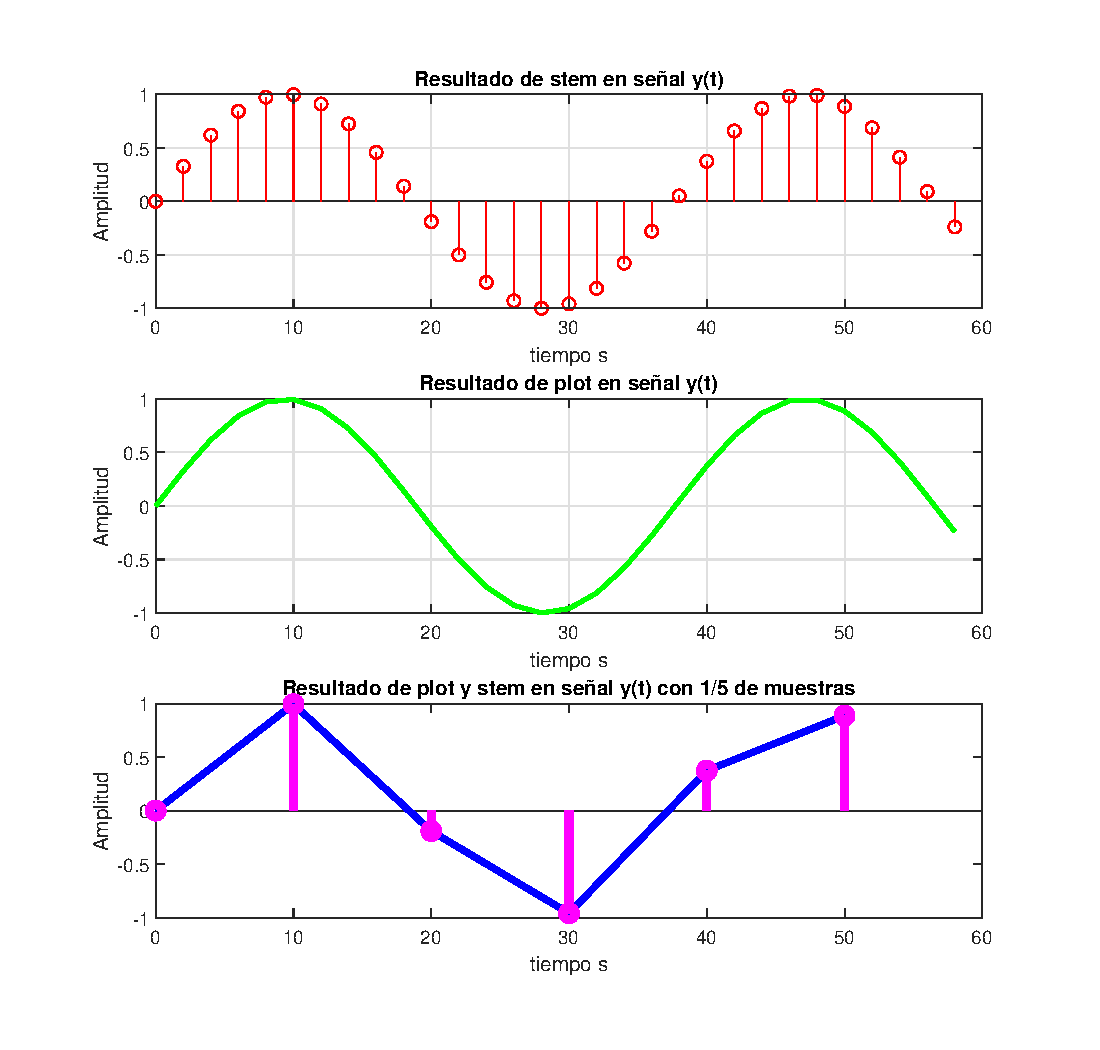
\includegraphics[scale = 0.8]{Imagenes/representacion_sennales.eps}
    \caption{Resultado de  comandos \textit{plot} y \textit{stem} aplicados a la señal $sin(t/6)$ }
    \label{plot_stem}
\end{figure}




\begin{enumerate}

    \item La figura  \ref{plot_stem} presenta tres gráficos, el primero muestra el resultado obtenido al aplicar el comando \texttt{stem} a la señal $y(t)$ considerando 30 muestras; el segundo muestra el resultado de graficar la señal $y(t)$ utilizando el comando \texttt{plot};  el tercero muestra el resultado de aplicar el comando \texttt{stem} a la señal $y(t)$ considerando 6 muestras además de graficarla utilizando el comando \texttt{plot}.
    
    \item Se puede notar que en los gráficos en los que se utiliza el comando \texttt{stem},se logra una clara representación de tiempo discreto de la señal, generando un punto en los instantes en que se toma la muestra de esta, mientras que cuando se utiliza el comando \texttt{plot}, lo que se obtiene es una gráfica que simula una señal de tiempo continuo a pesar de que la señal original corresponde a tiempo discreto. Esto se ve claramente en el tercer gráfico de la figura \ref{plot_stem}, en donde a pesar que se redujo el número de muestras tomadas, por lo que el espacio entre ellas es mayor, el resultado que se tiene  con el comando \texttt{plot} es una señal continua  que pierde la forma original de la señal, mientras que con el comando \texttt{stem}, aún se puede recuperar parte de la información se la señal $y(t)$ muestreada.
    
    \item Cuando se obtienen 30 muestras de la señal, el resultado obtenido es una señal claramente discreta que preserva la forma de la señal original $y(t)$, mientras que en el caso en que se reduce el numero de muestras en cinco veces, si bien la forma no es tan explicita respecto a la señal original, el número de muestras es suficiente para cumplir el criterio de Nyquist por lo que de todas formas se puede recuperar la señal $y(t)$. Se puede concluir que tomar 30 muestras de la señal no es estrictamente necesario para la señal que se está trabajando.
    
    \item El intervalo de $[0:59]$, corresponde a una ventana de 60 unidades de tiempo. No se especifica sobre que unidad puede ser. %durante las cuales se puede analizar la señal $y(t)$, se puede interpretar como una ventana de 60 segundos.
    
    %5
    \item 
    
    %Ambas señales tienen una duración de 60s, asumiendo que $t$ corresponde un intervalo de 1 minuto. Lo que cambia las señales discretas es el periodo de muestreo.
    
    No tiene sentido hablar de duración en segundos y frecuencia en Hz si no se conoce el periodo de muestreo.
    
    Siendo la frecuencia de muestro $f_s$, la duración en segundos de la primera sinusoide correspondería a:
    $$ \text{Duración} = \dfrac{60}{f_s}$$
    
    La frecuencia de la sinusoide discreta corresponde a la frecuencia relativa ($f_r$). A partir de la expresión para la frecuencia relativa se concluye que:
    $$ f_r = \dfrac{f}{f_s} \Rightarrow f = f_r\cdot f_s$$
    Por lo tanto para la primera sinusoide la frecuencia en Hz corresponde a:
    $$f = \dfrac{1}{2\pi}\cdot \dfrac{1}{6} f_s$$.
    
    La duración y frecuencia de la segunda sinusoide coincidiría con la primera, asumiendo una nueva frecuencia de muestreo acorde a un downsampling con un factor de 5.
    %No tiene sentido hablar de duración en segundos y Hz de una señal digital sin antes pasarla por DAC y un filtro. Para contestar la duración en tiempo y Hz se asumirá un retentor de orden cero para pasar de la discreta a la señal de tiempo continuo.
    
    %De esta ambas señales duran 60s y no serían periódicas.
    
    %No se cumple la periodicidad por no interpolar correctamente (el teorema del muestreo implica reconstrucción perfecta interpolando con funciones $ sinc $ ).
    

%\begin{table}[htbp]
%\begin{center}
%%\begin{tabular}{|l|l|l|}
%%%\hline
%%Señal  & Duracion [s]  & frecuencia [Hz] \\
%\hline \hline

%Señal muestreada con $n = 30$   &  \hspace{0.7cm}    2   & $\frac{6}{10}$\\ \hline

%Señal muestreada con $n = \frac{30}{5}$ & \hspace{0.7cm}  10  & $\frac{1}{10}$ \\ \hline

%\end{tabular}
%\caption{Duración en s y  frecuencia en Hz de las señales obtenidas.}
%\label{duracion_frec}
%\end{center}
%\end{table}

    
    \item El comando \texttt{stairs} asi como el comando \texttt{stem} o el comando \texttt{plot}, genera una figura en MATLAB que grafica una interpretación de la señal que se le ingresa como parámetro. Este comando en particular, a diferencia de \texttt{plot}, genera puntos cada vez que lee una muestra del vector/señal, e interpola generando puntos que conservan el valor de la última muestra hasta que lee una nueva muestra y repite el proceso, es decir, este comando se comporta como un circuito retentor de orden cero, o como un flip flop, ya que toma un valor y lo mantiene constante hasta tomar otro nuevo.
    
    En la figura \ref{stairs} se muestra una comparativa entre el uso del comando \texttt{plot} y el comando \texttt{stairs()}.
    
    \begin{figure}[H]
        \centering
        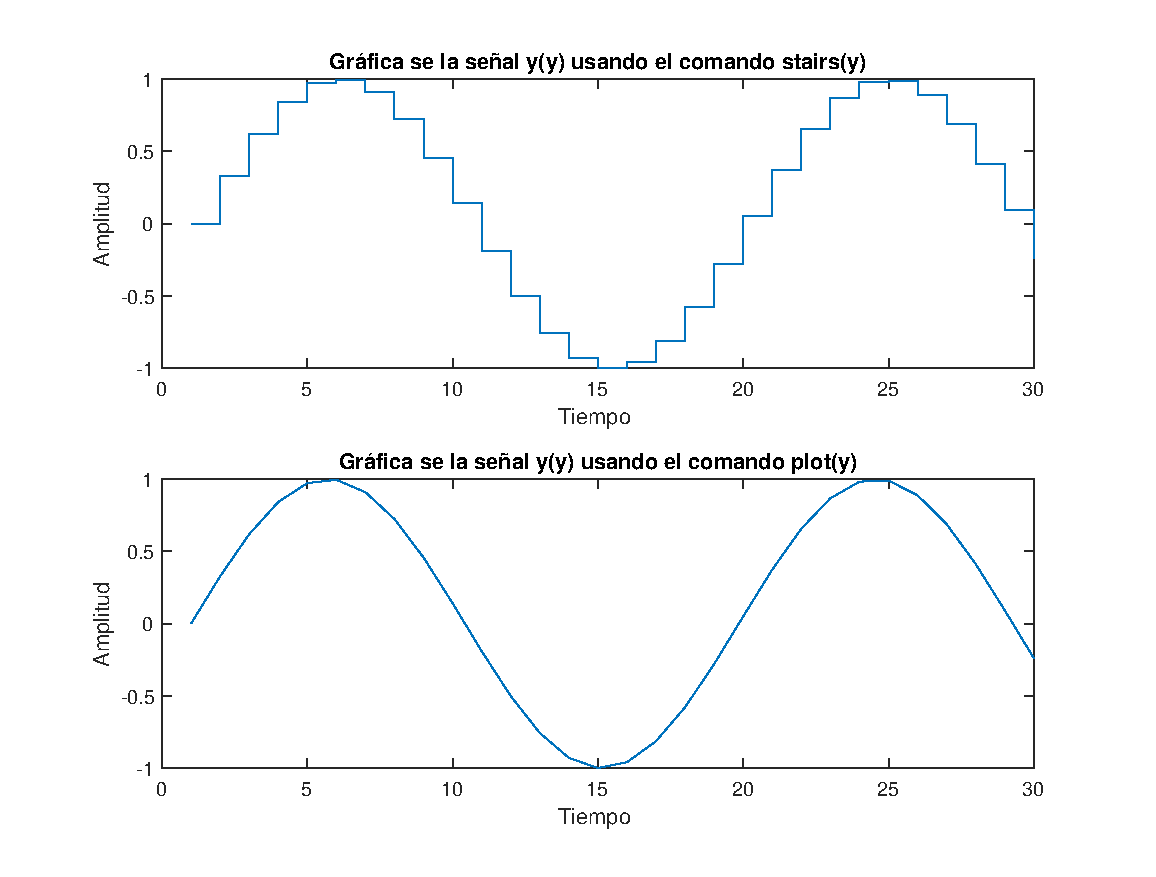
\includegraphics[scale = 0.6]{Imagenes/stairs.eps}
        \caption{Gráfica de la señal y(t) usando los comandos \texttt{plot} y el comando \texttt{stairs()}}
        \label{stairs}
    \end{figure}
    
    
    
    
    
\end{enumerate}


\subsection{Muestreo}

Para esta sección se considera la señal de tiempo continuo $s(t) = sin(2\pi t)$, muestreada a intervalos uniformes $T_s$.

\begin{enumerate}
    
    %1
    \item Usando $T_s = 1/10$ y $ 0 \leq n \leq 100 $ se tiene:
    $$s_1[n] = \sin\left(2\pi \dfrac{1}{10}n\right)$$
    cuyo gráfico utilizando el comando \texttt{stem} se muestra en la figura \ref{fig:Ip2}.
    
    %2
    \item Usando $T_s = 1/3$ y $ 0 \leq n \leq 30 $ se tiene:
    $$s_2[n] = \sin\left(2\pi \dfrac{1}{3}n\right)$$
    cuyo gráfico utilizando el comando \texttt{stem} se muestra en la figura \ref{fig:Ip2}.
    
    %3
    \item Usando $T_s = 1/2$ y $ 0 \leq n \leq 20 $ se tiene:
    $$s_3[n] = \sin\left(2\pi \dfrac{1}{2}n\right)$$
    cuyo gráfico utilizando el comando \texttt{stem} se muestra en la figura \ref{fig:Ip2}.
    
    %4
    \item Usando $T_s = 10/9$ y $ 0 \leq n \leq 9 $ se tiene:
    $$s_4[n] = \sin\left(2\pi \dfrac{10}{9}n\right)$$
    cuyo gráfico utilizando el comando \texttt{stem} se muestra en la figura \ref{fig:Ip2}.
    
    \begin{figure}[H]
    \centering
    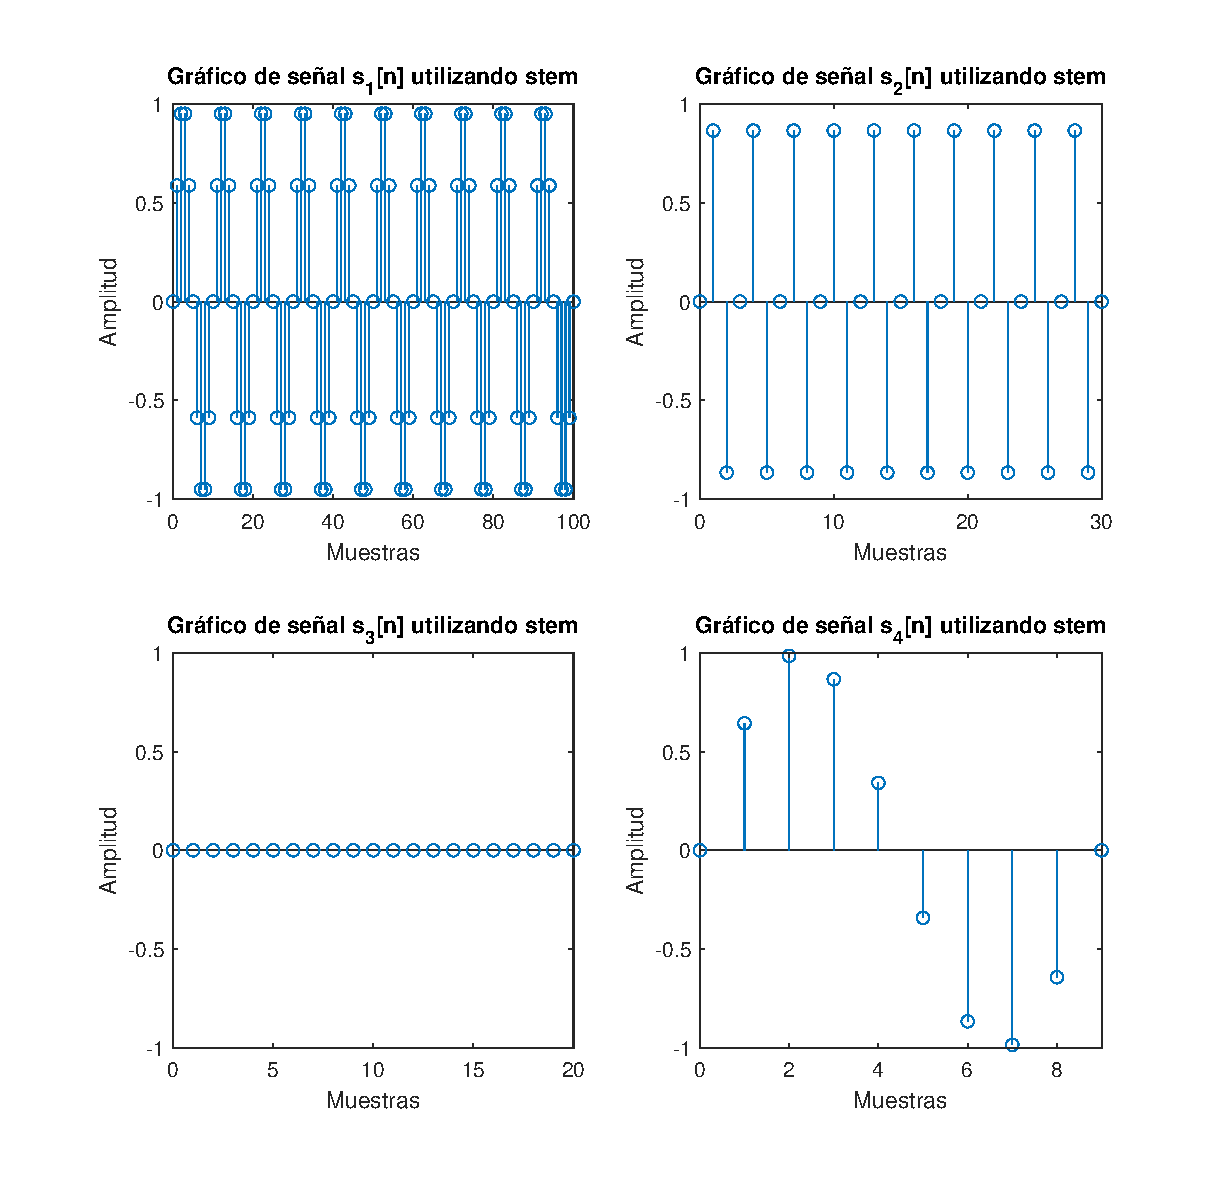
\includegraphics[scale = 0.7]{Imagenes/muestreo_sennales.eps}
    \caption{Señales de tiempo discreto $s_1[n]$, $s_2[n]$, $s_3[n]$ y $s_4[n]$.}
    \label{fig:Ip2}
    \end{figure}
    
    %5
    \item La frecuencia de cada señal de tiempo discreto en ciclos por muestra corresponde a:
    $$ f_r = f \cdot T_s = T_s$$
    donde $f$ corresponde a la frecuencia de la señal de tiempo continuo.
    Por lo anterior la frecuencia de las señales de tiempo discreto obtenidas son:
    
    \begin{itemize}
        \item $s_1[n]$: $1/10$ ciclos por muestra.
        \item $s_2[n]$: $1/3$ ciclos por muestra.
        \item $s_3[n]$: $1/2$ ciclos por muestra. 
        \item $s_4[n]$: $10/9$ ciclos por muestra.
    \end{itemize}
    
    %6
    \item Las muestras por periodo, considerando un periodo de 1 s en la señal de tiempo continuo, corresponde a:
    $$ \text{muestras por periodo}  = \dfrac{T}{T_s} = \dfrac{1 s}{ T_s} $$
    donde $f$ corresponde a la frecuencia (Hz) en tiempo continuo. De lo anterior se concluye que:
    
    \begin{itemize}
        \item $s_1[n]$: 10 muestras por periodo
        \item $s_2[n]$: 3 muestras por periodo
        \item $s_3[n]$: 2 muestras por periodo
        \item $s_4[n]$: 0.9 muestras por periodo.
    \end{itemize}
    
    %7
    \item En términos de series de tiempo, claramente las señales no son equivalentes, pues son secuencias distintas pues tienen valores numéricos distintos para los mismos valores del eje x.
    
    En términos de reconstrucción de la señal de tiempo continuo, las señales $s_1[n]$ y $s_2[n]$ son equivalentes, pues cumplen el criterio de nyquist.
    
    %8
    \item La frecuencia de muestreo $f_s$ (sps) que generan cada una de las señales corresponde a:
    $$ f_s = 1/T_s$$
    de lo anterior se concluye que:
    
    \begin{itemize}
        \item $s_1[n]$: 10 sps
        \item $s_2[n]$: 3 sps
        \item $s_3[n]$: 2 sps
        \item $s_4[n]$: 0.9 sps
    \end{itemize}
    
    lo que numéricamente coincide con las muestras por periodo. Esto es debido a que el periodo de la señal de tiempo continuo es de 1 segundo.
    
    %9
    \item La resolución de muestreo afecta a la frecuencia de la señal de tiempo discreto ($f_r$) de la siguiente forma:
    $$ f_r = f/f_s$$
    donde $f$ corresponde a la frecuencia de la señal en tiempo continuo y $f_s$ a la frecuencia de muestreo.
    
    Mas importante que la expresión anterior es el doblaje de frecuencias, donde al no cumplir estrictamente el criterio de nyquist, es decir:
    
    $$ f_r \leq 0.5$$
    
    no se es capaz de distinguir la frecuencia de la señal de tiempo continuo con respecto a otra en el intervalo $[0 ; f_s/2]$.
    
    Dicho efecto ocurre en la señal $s_4[n]$. Aquí $f_s$ es mayor a las demás señales (observar parte 5.) sin embargo, en la figura \ref{fig:Ip2} se observa una frecuencia menor. 
    
    Para obtener la frecuencia observada en $s_4[n]$ ($f_{\text{obs}}$) se calcula:
    
    $$ f_{\text{obs}} = (f_r - 1) = \dfrac{10}{9}-1 = 1/9 $$
    
    expresión que se concluyó a partir del diagrama de doblaje de frecuencias, mostrado en la figura \ref{fig:Ip2df}.
    
    \begin{figure}[H]
        \centering
        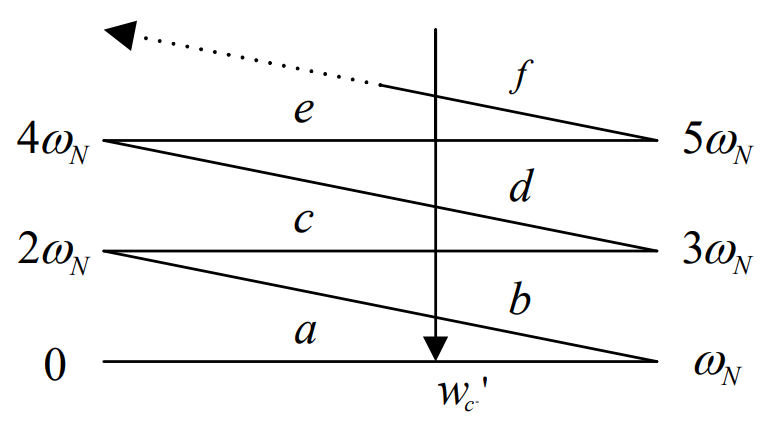
\includegraphics[width = .6 \linewidth]{Imagenes/Ip2_df.png}
        \caption{Diagrama de doblaje en frecuencias.}
        \label{fig:Ip2df}
    \end{figure}
    
    Cabe mencionar que el efecto en $s_3[n]$ de observar una frecuencia de 0 ciclos por muestra no corresponde a doblaje en frecuencia, sino que es debido a la fase de la sinusoide y a no cumplir el criterio de Nyquist.
    
    
    

    
\end{enumerate}





%---------------Generación de señales------------------
\subsection{Generación de señales}

Se considera la función senoidal $s(t) = Asin(2\pi ~f~t + \phi)$, donde A es la amplitud de la señal, $t$ es el tiempo en segundos, $f$ es la frecuencia en Hz y $\phi$ la fase de la señal en radianes. Se buscará generar la función de tiempo discreto $s[n] = Asin(2\pi (f/f_s)n + \phi)$, donde $f_s$ es la frecuencia de muestreo en \textit{sps},  y $n~\in \left\lbrace \mathbb{N} + 0 \right\rbrace\ $

\begin{enumerate}
    \item Se generan dos señales sinusoidales de frecuencias $50~Hz$ y $500~Hz$, con duración de $1~seg$, la misma fase inicial y amplitud unitaria.
    
    Se escoge una frecuencia de muestreo $f_s = 4~kHz$, dado que este valor cumple holgadamente el criterio de Nyquist según el teorema del Muestreo, además cumple también este criterio para trabajar las frecuencias presentes en actividades posteriores.
    
    La figura \ref{s50_s500} muestra las gráficas obtenidas usando el comando \texttt{plot} a las señales  de frecuencias $50~Hz$ y $500~Hz$, antes mencionadas.
    
    \begin{figure}[H]
        \centering
        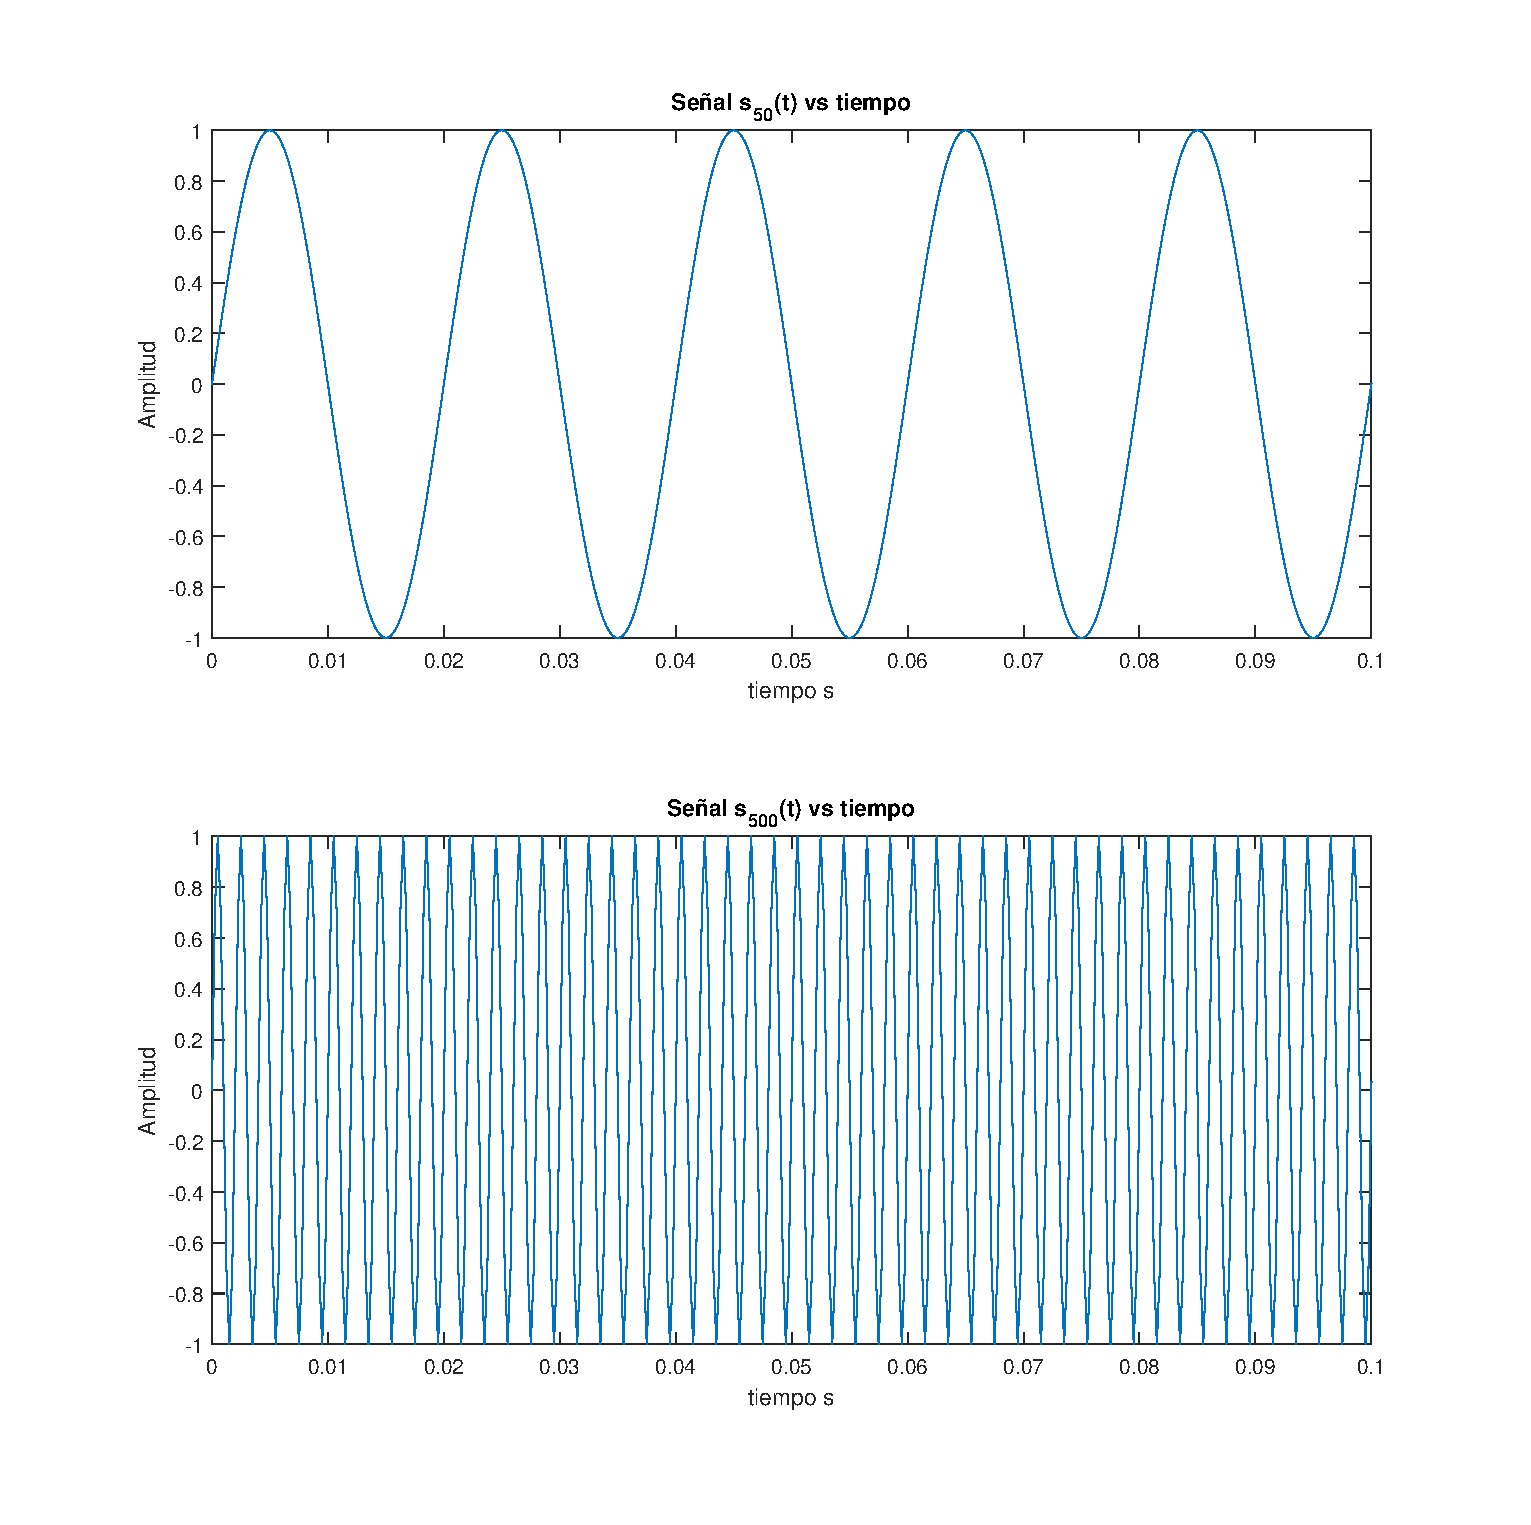
\includegraphics[scale = 0.6]{Imagenes/s50_s500.eps}
        \caption{Gráfica de las señales sinusoidales de  de frecuencias $50~Hz$ y $500~Hz$ generadas.}
        \label{s50_s500}
    \end{figure}
    
    Al reproducir estas señales con el comando \texttt{soundsc}, se puede notar que la señal de frecuencia $50~Hz$  es apenas audible, mientras que la que tiene una frecuencia de $500~Hz$  se logra percibir claramente como un tono puro.
    
    
    \item   Al hacer la suma las dos señales generadas de frecuencias $50~Hz$ y $500~Hz$, se obtiene una señal de $500~Hz$ montada sobre una señal de $50~Hz$, es decir, esta señal resultante conserva el periodo de su componente de menor frecuencia, en este caso $0.02~s$ Esto se puede ver en la primera gráfica de la figura \ref{suma_senos}
    
    
    Al realizar esta misma prueba de sumar dos señales sinusoidales, pero esta vez siendo de frecuencias de $200~Hz$ y  $300~Hz$, Lo que se obtiene es una señal que mezcla ambas componentes,  pero con un periodo de $0.01~s$, como se ve en la segunda gráfica de la figura \ref{suma_senos} Se empieza a notar el comportamiento de una señal generada por la suma de dos sinusoides, donde la frecuencia fundamental de esta señal resultante corresponde al máximo común divisor entre las frecuencias de las componentes de la señal, siendo en este caso de $100~Hz$
    
    Finalmente al componer el acorde de \textit{LA}, sumando tres señales sinusoidales con frecuencias de $880~Hz$, $100~Hz$ y $1320~Hz$ se deduce que la señal resultante deberá tener como frecuencia fundamental el máximo común divisor entre las frecuencias que la componen, en este caso de $220~Hz$, por lo que se tiene que las  frecuencias utilizadas corresponden a los armónicos 4,5 y 6 respectivamente de la nota LA2.
    
    
    Al reproducir la primera señal generada, en donde una de sus componentes coincide con la frecuencia fundamental resultante lo que se escucha son dos tonos por separado, mientras que en los dos últimos casos, donde la frecuencia fundamental resultante no se encuentra entre las componentes que la formaron se escucha un sonido más homogéneo.
    
    \begin{figure}[H]
        \centering
        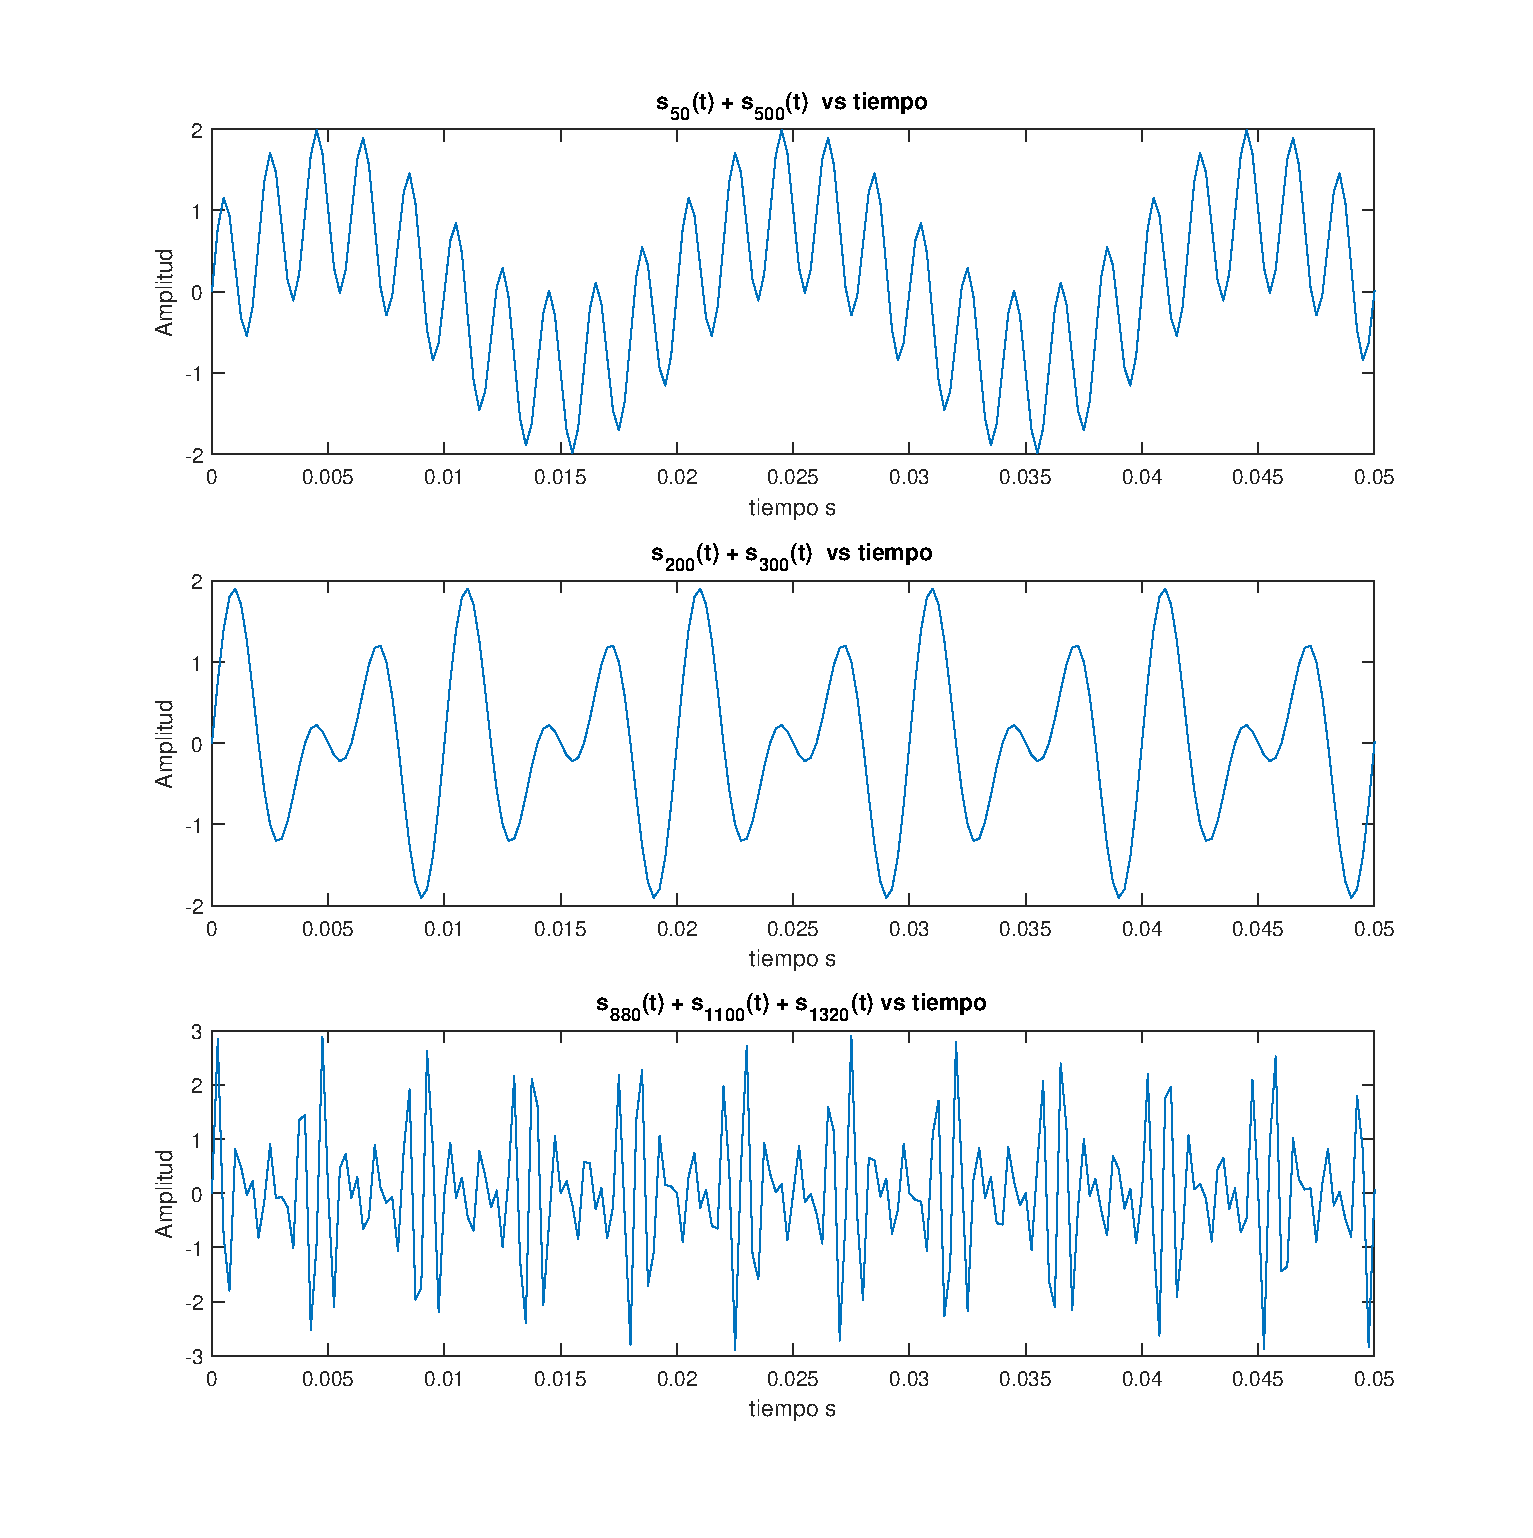
\includegraphics[scale = 0.6]{Imagenes/suma_senos.eps}
        \caption{Gráficas de las señales obtenidas mediante suma de tonos puros.}
        \label{suma_senos}
    \end{figure}
    
    %3
    \item Se desarrolla un  script para sintetizar una aproximación de una señal cuadrada mediante  una componente sinusoidal fundamental sumada a sus armónicos impares desde el 3 al 11, esto considerando fase igual a cero. Siguiendo la expresión siguiente:
    
    
    $$ ss[n] = \sum^6_{k=1} sin(2\pi (2k-1)(f/f_s)n)$$
    
    Obteniendo de esta mandera, la gráfica presente en la figura \ref{sint_fase0}, incrementando cada vez un armónico impar a la serie finita.
    
    \begin{figure}[H]
        \centering
        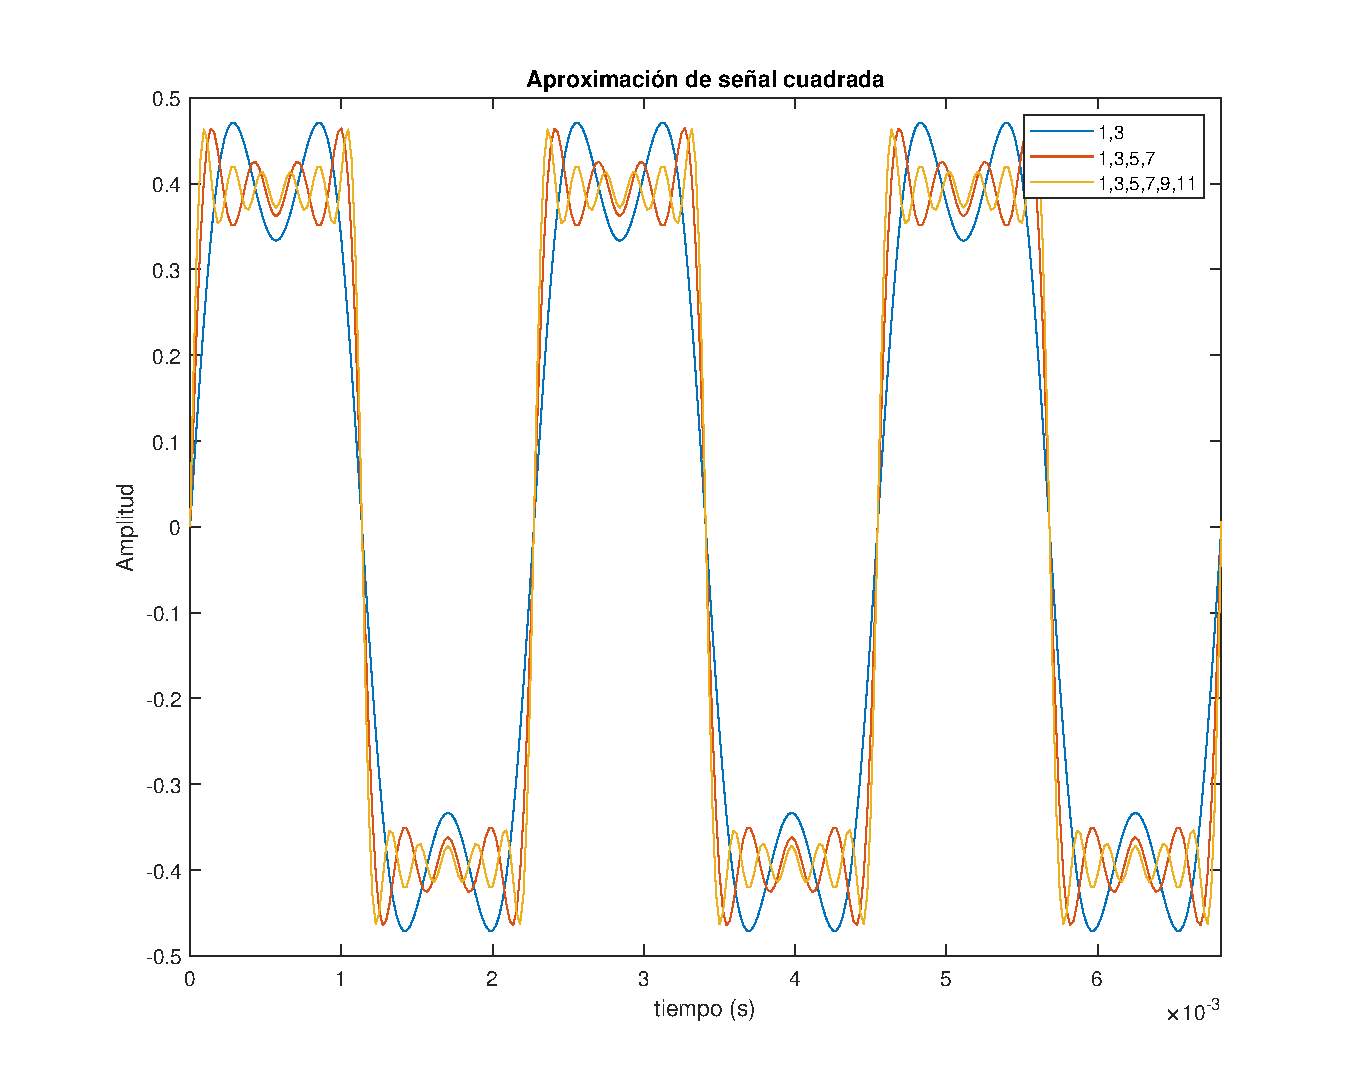
\includegraphics[scale = 0.5]{Imagenes/aproximacion_sennal_cuadrada.eps}
        \caption{Aproximación sintetizada con sinusoidal fundamental y armónicos impares del 3 a 11}
        \label{sint_fase0}
    \end{figure}
    
Luego se modifica el script para poder añadir una fase aleatoria a la aproximación de la señal, siguiendo la siguiente expresión:
    $$ ss[n] = \sum^6_{k=1} sin(2\pi (2k-1)(f/f_s)n + \phi (k))$$


Los resultados de ambos casos se muestran en la figura \ref{sintetizadas}

\begin{figure}[H]
    \centering
    \includegraphics[scale = 0.5]{Imagenes/aprox_cuadrada-armónicos_fase_al.eps}
    \caption{Aproximación sintetizada mediante armónicos tanto con fase cero como con fase aleatoria.}
    \label{sintetizadas}
\end{figure}
    
    
    Para ambas situaciones se utilizó una frecuencia de muestreo de $44~kHz$ para asegurar que se cumpla el criterio de Nyquist para todas las frecuencias presentes en estos experimentos. 
    \newline
    Como se puede apreciar en la figura \ref{sintetizadas} el cambio de fase de las componentes provoca un notorio cambio en la forma de onda de la señal resultante, dejando de acercarse a lo que es una señal cuadrada. Sin embargo,  la frecuencia de ambas señales resultantes (o tono, hablando sobre lo audible) se conserva. 
    En cuanto a la percepción, como ya se mencionó el tono escuchado es el mismo pero el timbre del sonido es ligeramente distinto cuando las formas de ondas obtenidas en fase cero y fase aleatoria son similares, pero en otros casos la forma de onda de la señal generada con fase aleatoria difiere significativamente respecto a la que tiene fase cero, en estas ocasiones el timbre era notablemente distinto entre ambos sonidos.
    
    
    
    
    %4
    \item Se generan señales aleatorias de distribución uniforme en el intervalo $[-1; 1]$ utilizando distintas frecuencias de muestro (2, 10 y 44 kHz), las cuales son usadas como ruido aditivo a la señal discreta obtenida a partir del muestreo de la señal original $\sin(2\pi 500 t)$. Los gráficos de las señales se muestran en la figura \ref{fig:p4}.
    
    \begin{figure}[H]
        \centering
        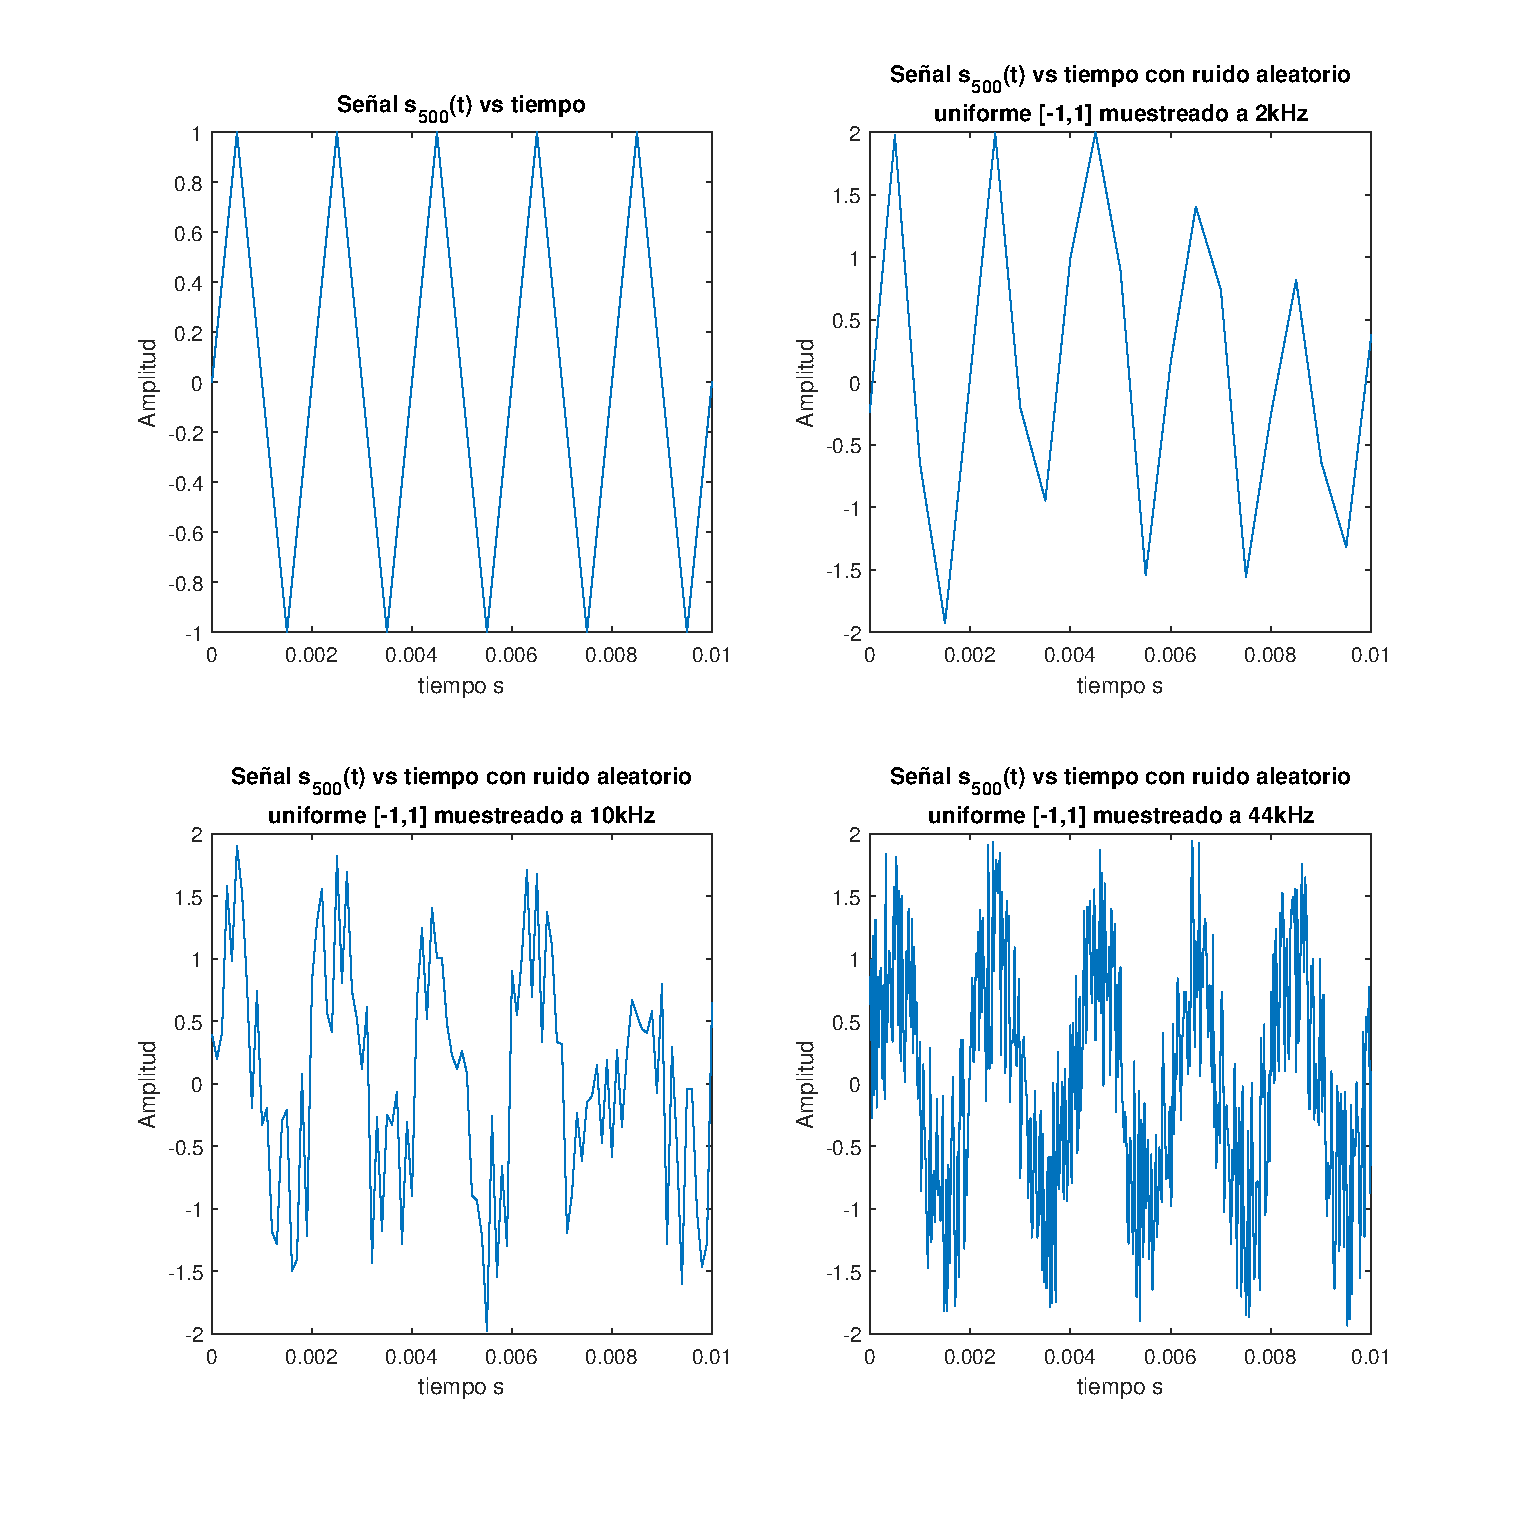
\includegraphics[width = .6\linewidth ]{Imagenes/p4.eps}
        \caption{Primeros 10 ms de señal sinusoidal original y señal generada con amplitud aleatoria.}
        \label{fig:p4}
    \end{figure}
    
    En la figura \ref{fig:p4} se aprecia que a medida que la frecuencia de muestreo aumenta el ruido se hace más evidente. Lo anterior se le atribuye al doblaje en frecuencias ya que a medida que la frecuencia de muestreo aumenta se logra distinguir ruido de alta frecuencia. Se concluye que muestrear a sobretasa (en términos de Nyquist) para una señal que presenta ruido aditivo puede ser contraproducente.
    
    %5
    \item Se pide modificar la señal sinusoidal original de 500 Hz de modo que la amplitud varíe aleatoriamente entre $[0.5;1]$. Se utiliza una distribución uniforme en este intervalo.
    
    El gráfico de los primeros 10 ms de la nueva señal y original se muestra en \ref{fig:p5}.
    
    \begin{figure}[H]
        \centering
        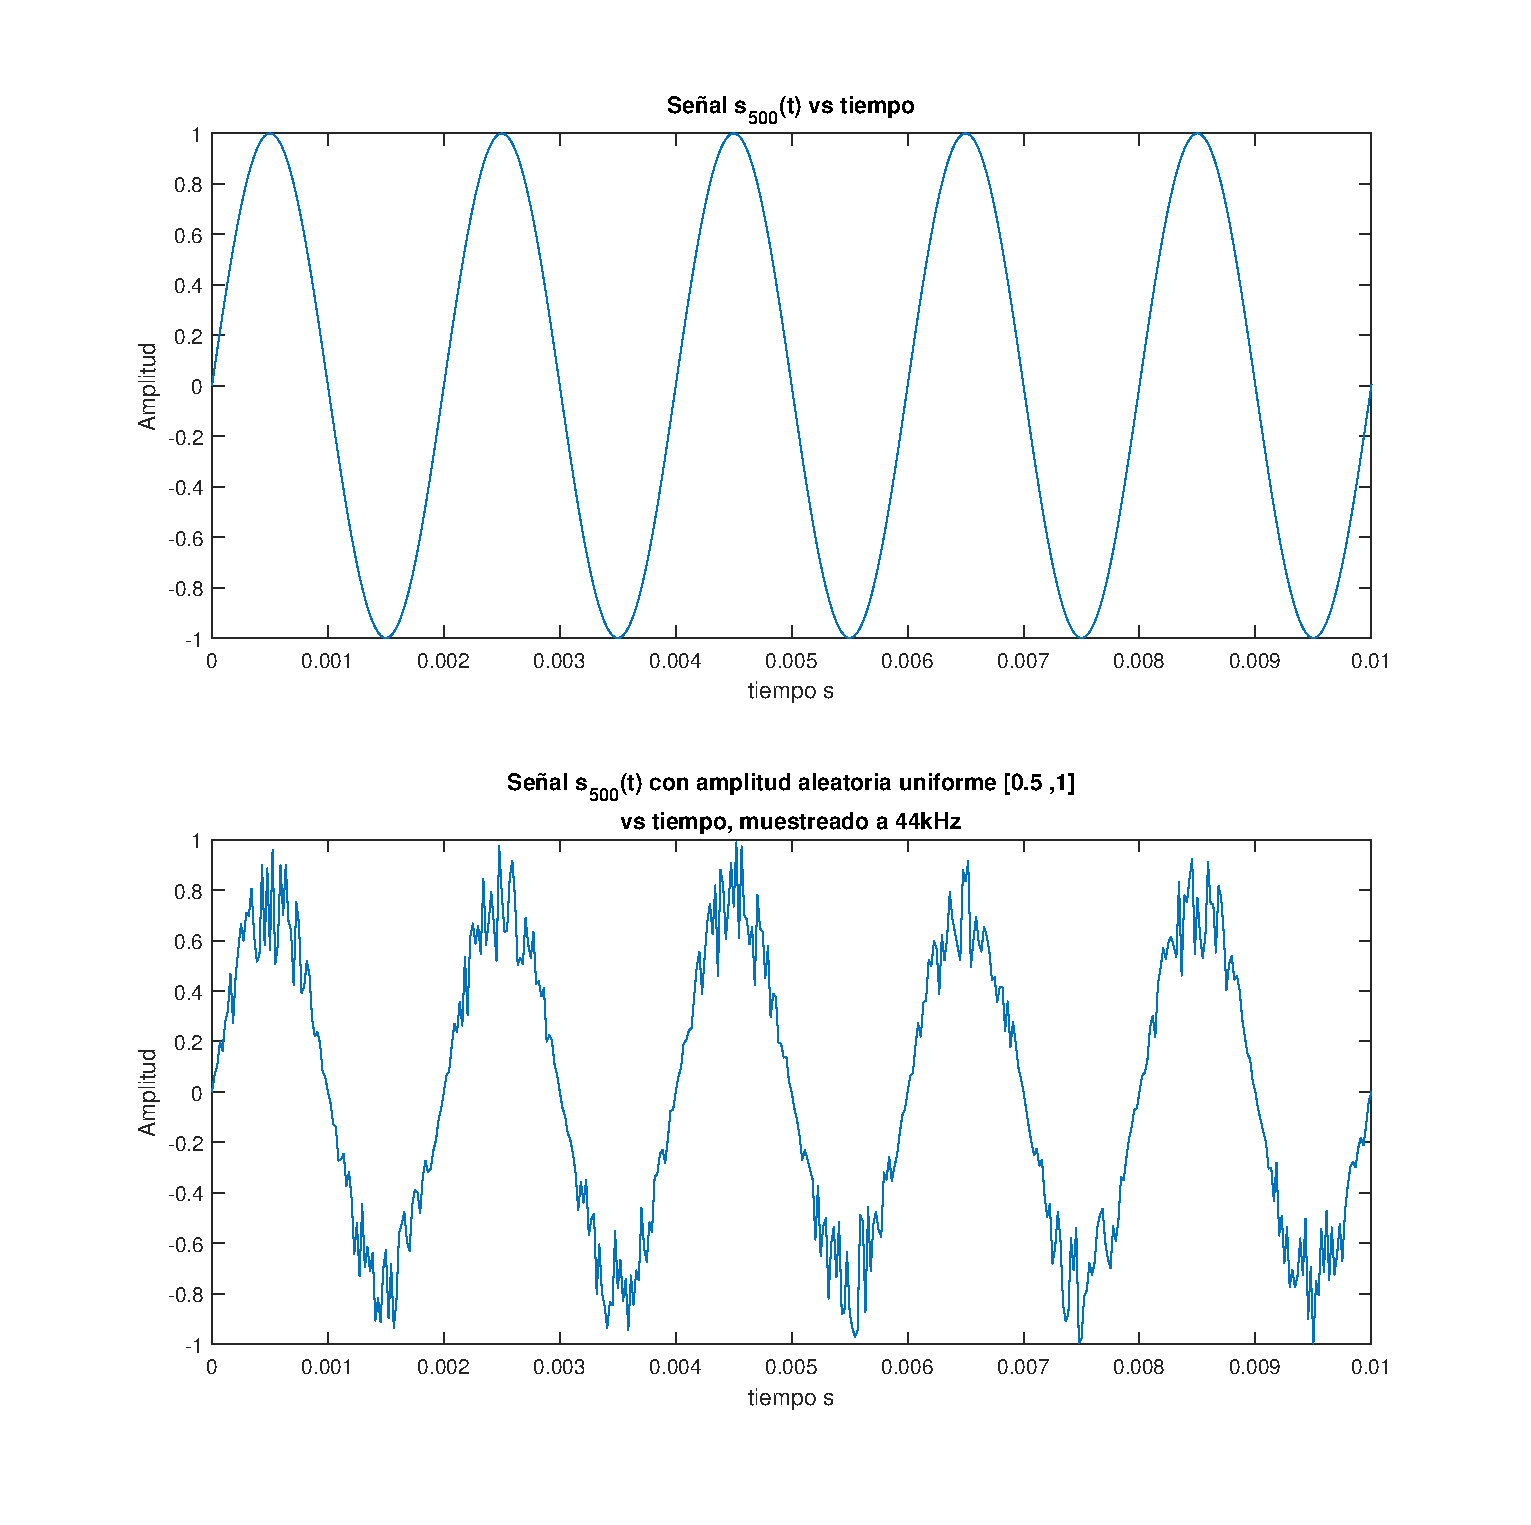
\includegraphics[width = .6\linewidth ]{Imagenes/p5.eps}
        \caption{Primeros 10 ms de señal sinusoidal original y señal generada con amplitud aleatoria.}
        \label{fig:p5}
    \end{figure}
    
    %6
    \item Se pide modificar la señal sinusoidal original de 500 Hz de modo que su fase varíe aleatoriamente entre $[\pi/2;\pi/2]$. Se utiliza una distribución uniforme en este intervalo.
    
    El gráfico de los primeros 10 ms de la nueva señal y original se muestra en \ref{fig:p6}.
    
    \begin{figure}[H]
        \centering
        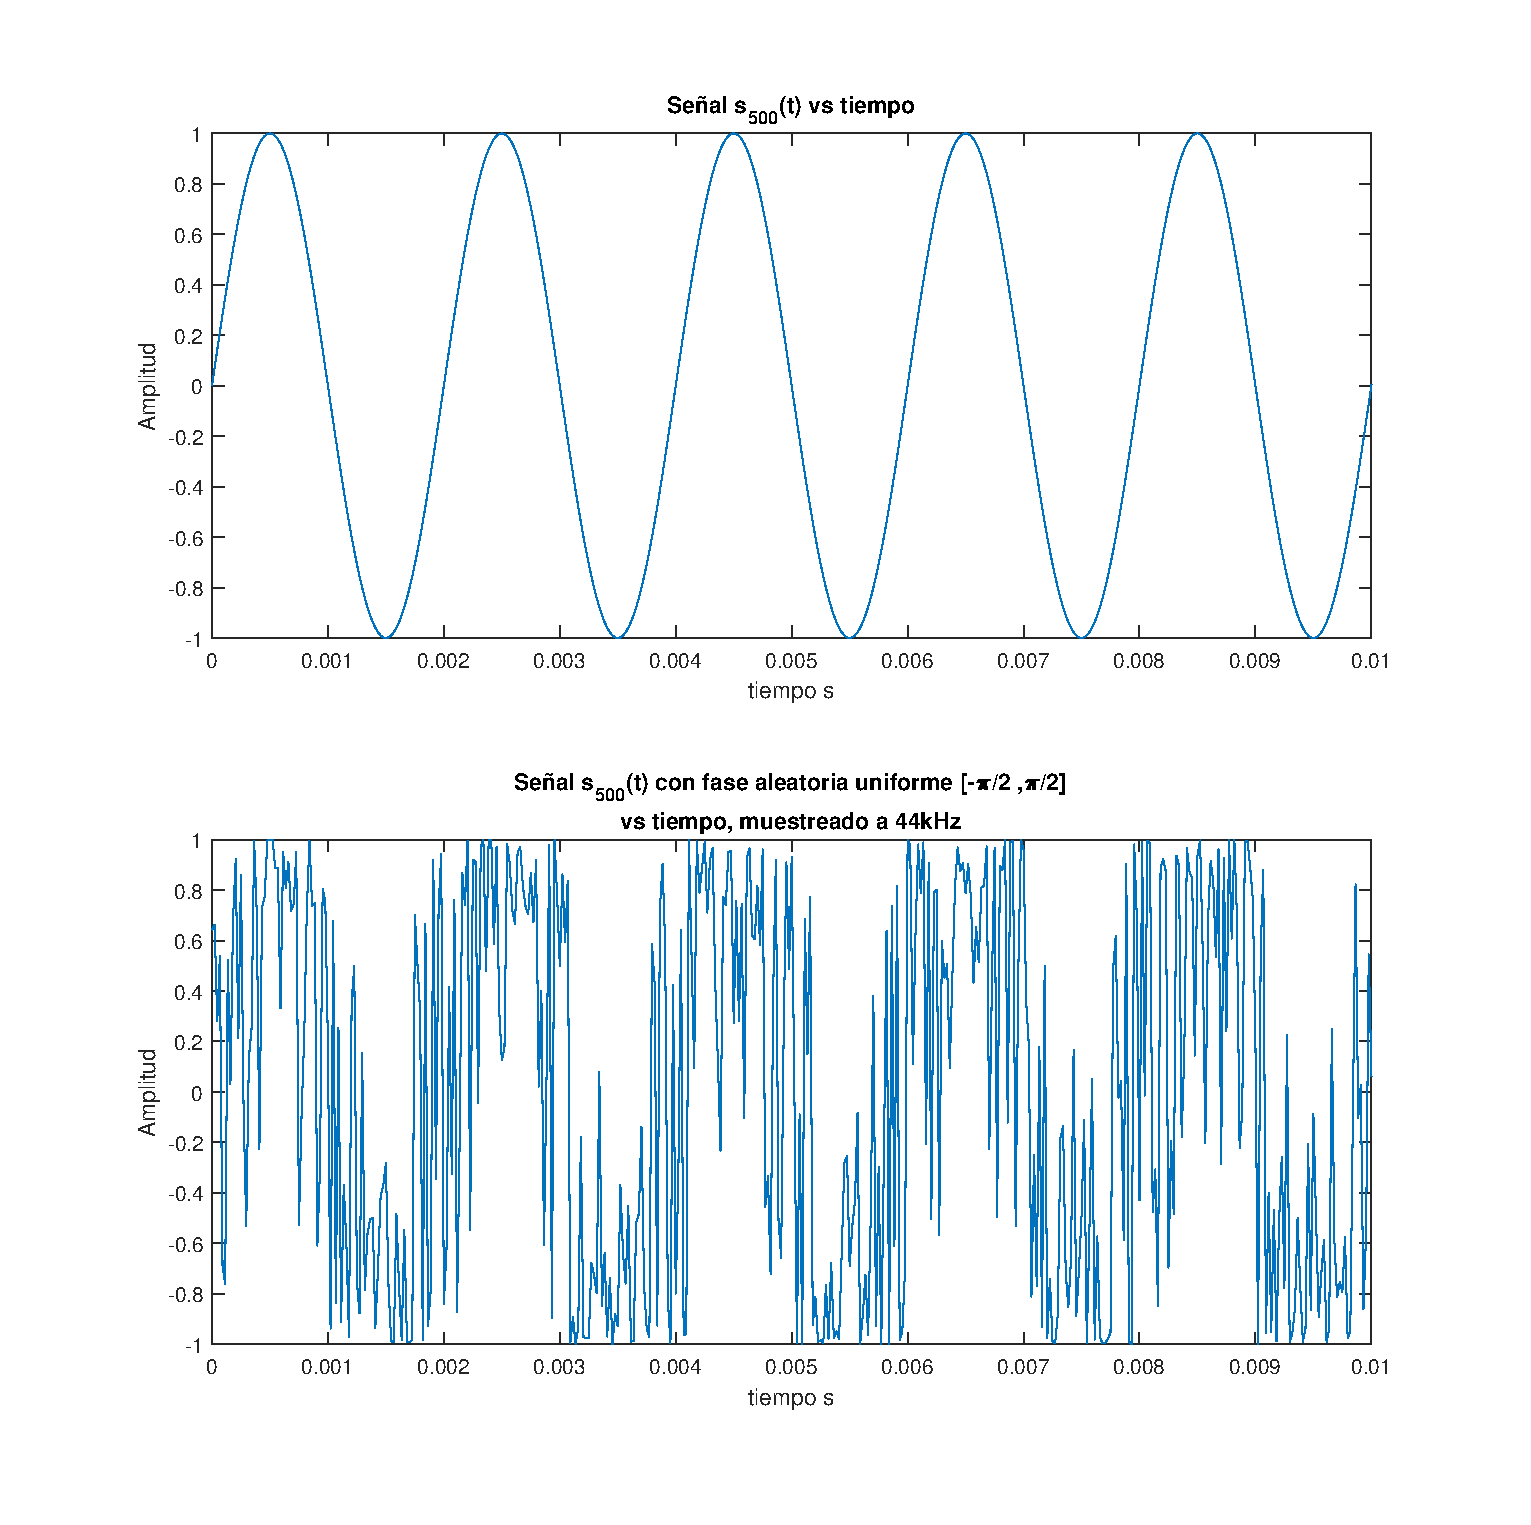
\includegraphics[width = .6\linewidth ]{Imagenes/p6.eps}
        \caption{Primeros 10 ms de señal sinusoidal original y señal generada con fase aleatoria.}
        \label{fig:p6}
    \end{figure} 
    
    %7
    \item Con respecto a los tipos de ruido con los que se experimentó en los puntos anteriores, se observa que:
    \begin{itemize}
        \item El ruido aditivo afecta a los valores puntuales de la señal, sin emargo, visualmente la frecuencia de la señal es distinguible. Esta propiedad es interesante al pensar en modulación FM en un canal. 
        
        
        \item El ruido en amplitud resulta visualmente evidente cuando el valor de la señal sinusoidal es alto. Comparativamente es el menos dañino para la señal original. 
        
        \item La fase aleatoria es, comparativamente, el tipo de ruido que genera mayor deformación de la señal original.
    \end{itemize}
    
    Con respecto a la percepción auditiva de las señales generadas se puede comentar que:
    
    \begin{itemize}
        \item Para los audios generados con ruido aditivo, a medida que se aumenta la frecuencia de muestreo el ruido se vuelve más ''rico'' en frecuencias. Sintiendose grave para 2 kHz y molestamente agudo a 44 kHz.
        
        \item La amplitud aleatoria genera el ruido mas suave sobre la señal original, como se esperaba del análisis visual.
        
        \item La fase aleatoria genera un ruido perceptualmente similar la aditiva, sin embargo, la razón perceptual entre el ruido y la señal original es claramente mayor que en el caso aditivo. Probablemente la SNR en esta señal es menor.
    \end{itemize}
    
    
    
    
    
    
    
    
\end{enumerate}

\clearpage
\section{Parte Complementaria}


\subsection{Experimento doblaje}
\begin{enumerate}
    \item Al reproducir el archivo de audio original, se logra apreciar la mezcla de dos componentes, una de estas componentes se mantiene constante, se agudiza despeas de un momento, se vuelve a mantener constante en ese tono y  se agudiza nuevamente para mantenerse en constante en ese último tono, es decir, cada vez que se agudizó la señal aumentó su frecuencia; mientras la otra componente se vuelve más aguda, o aumenta su frecuencia,  de forma lineal en tres oportunidades comenzando su incremento en el mismo instante en que la componente constante se agudiza. 
    
    Para el caso en que se reproduce una señal de audio que tiene la mitad del tamaño que tenía el archivo original, en el que se consideran solo muestras pares de dicho archivo, también se pueden distinguir dos componentes, una varía y la otra se mantiene constante tal como en el caso en que se reproduce la señal original. Sobre la componente que varía, se puede notar que esta al principio  aumenta linealmente su frecuencia igual que antes, pero en el segundo y tercer cambio que presenta la componente constante, la que varía posee un incremento lineal hasta que llega un punto en que el la variación corresponde a un  un decremento lineal en frecuencias, apreciándose como un sonido que se agudiza lentamente   y luego se torna cada vez mas grave.
    
    Finalmente, cuando se hace \textit{Downsampling} a la señal original tomando una de cada tres muestras almacenándolas en un vector que tiene un tercio del tamaño del archivo original, nuevamente se distinguen dos componentes, una componente que se mantiene constante presentando ligeros cambios después de unos instantes  igual que en los dos casos anteriores, o suena levemente más agudo, mientras que la otra componente en principio se hace cada vez mas aguda hasta que en un momento comienza a hacerse mas grave, es decir aumenta linealmente su frecuencia y luego decrece también linealmente, al presentarse el primer cambio en la componente constante, la componente que varía presenta un comportamiento similar al antes descrito,  pero esta vez el tiempo que se mantiene el incremento lineal es menor al tiempo  que dura el decrecimiento. Cuando se presenta la última modificación en la componente constante, se aprecia que  la componente que varía comienza aguda y el sonido solo se hace más grave decrementando linealmente su frecuencia.
    
    \item Lo descrito anteriormente, que corresponde a la apreciación auditiva de las señales obtenidas se puede corroborar viendo el espectrograma de las tres señales, la correspondiente al archivo de audio original, la que tiene sólo las muestras pares y la que se obtiene haciendo \textit{Downsampling} con $D = 3$
    
    
    \begin{figure}[H]
        \centering
        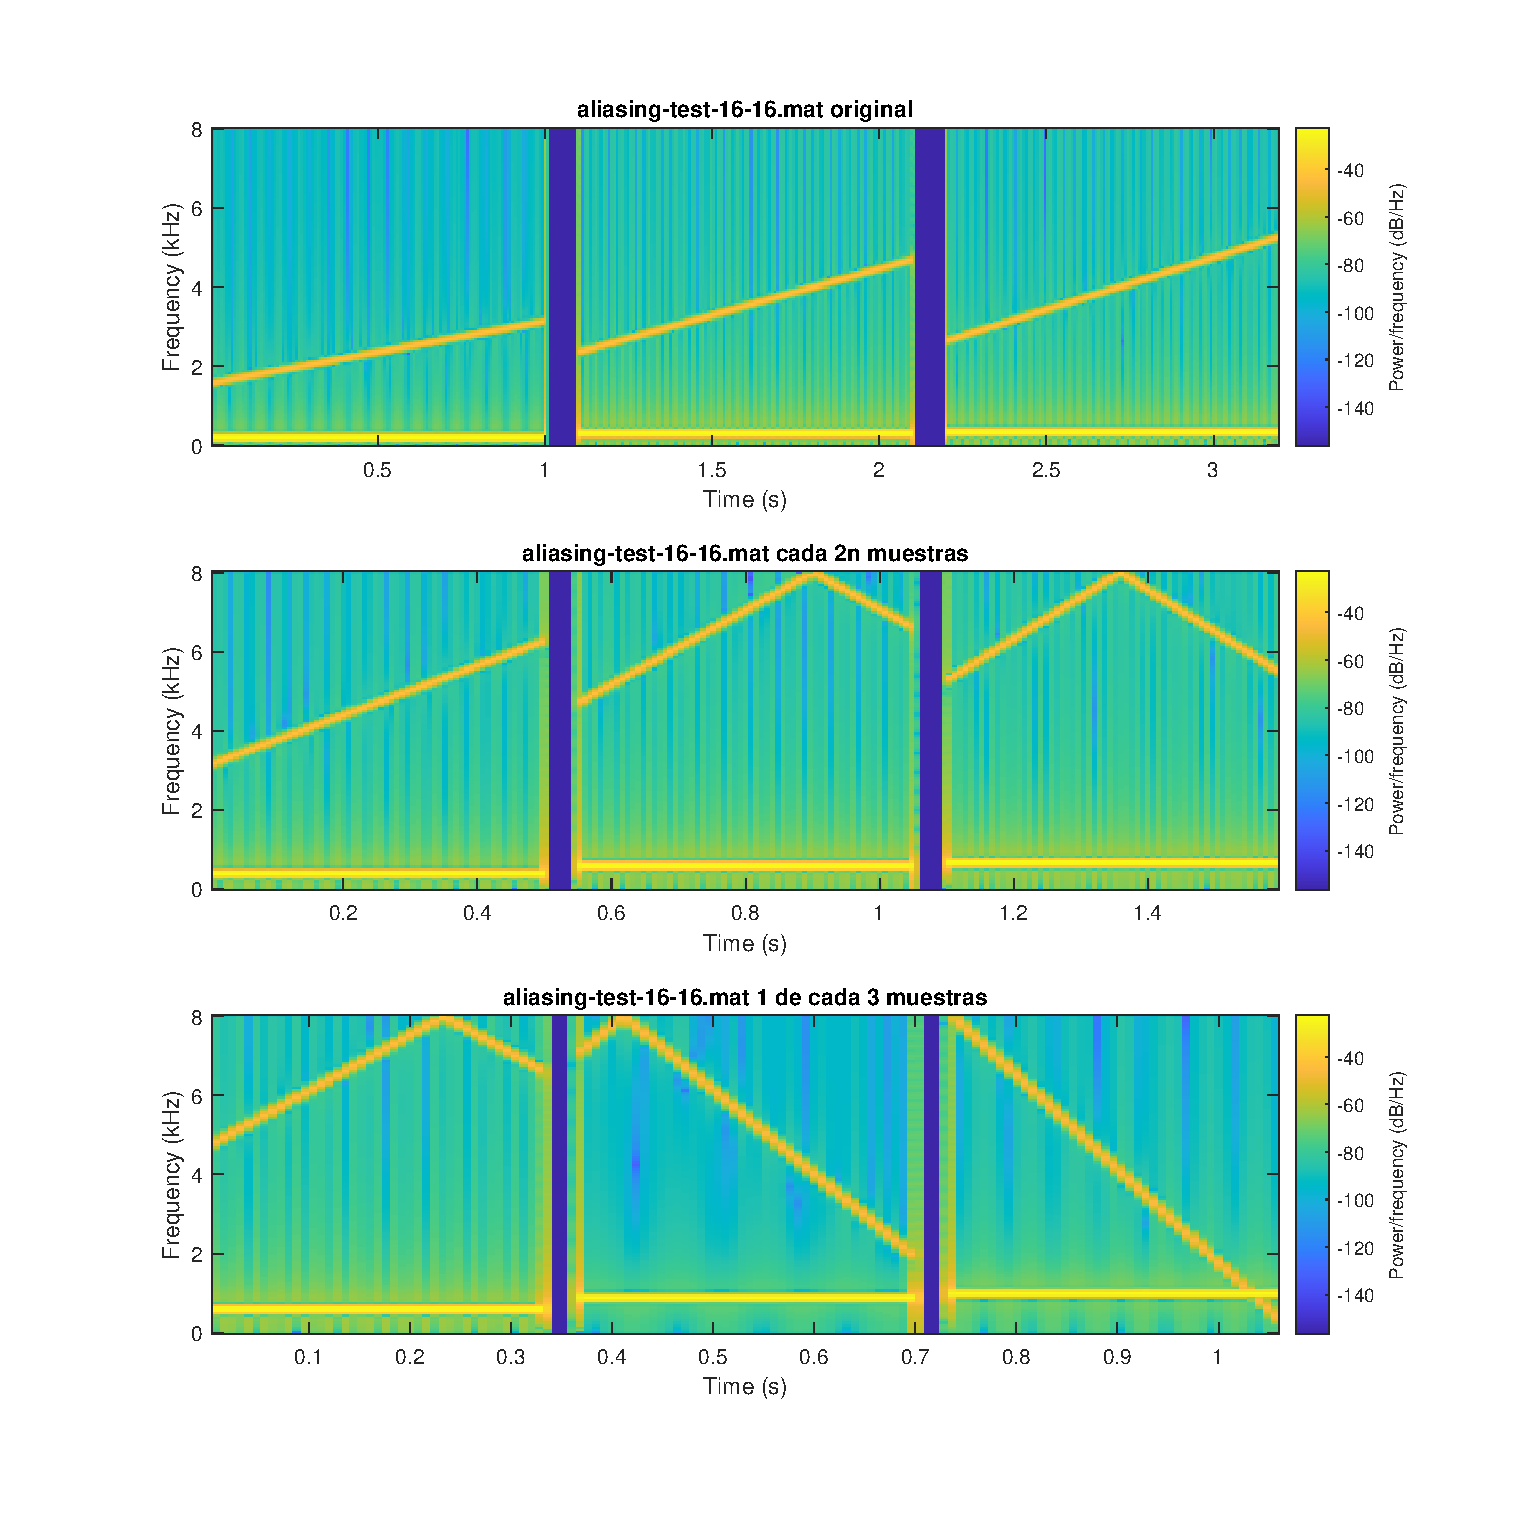
\includegraphics[scale = 0.5]{Imagenes/espectogramas.eps}
        \caption{Espectrograma de las señales obtenidas y reproducidas a partir del archivo de audio \texttt{aliasing-text-16-16}.}
        \label{fig:my_label}
    \end{figure}
    
    
    Observando el  espectrograma correspondiente al archivo de audio original, se puede deducir que la tasa mínima a la que se podría re-muestrear el vector de datos original es de al menos  de los $10.6~kHz$
\end{enumerate}


\subsection{Efectos de la cuantización en procesadores digitales }

\begin{enumerate}

\item 
    Se cargan los archivos de audio \texttt{sonidos-de-voz-16-16.wav} y \texttt{musica-16-16.wav} y se desarrolla la función \texttt{cuantiza(x,N)} en MATLAB para analizar qué tanto se distorsiona una señal de audio al ser cuantizada, y cómo influyen en este proceso la cantidad de bits que se utilizan para realizar dicha cuantización.
    
    \begin{figure}[H]
        \centering
        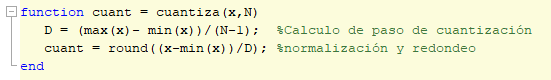
\includegraphics[scale = 0.7]{imagenes2/cuantiza.png}
        \caption{Implementación en MATLAB de la función \texttt{cuantiza}}
        \label{fig:cuantiza}
    \end{figure}
    
    En la figura \ref{fig:cuantiza} se tiene el código de implementación para una función que cuantiza una señal que se recibe con el parámetro \textit{x}  y donde \textit{N} corresponde a la cantidad de niveles de cuantización que se considerarán en el proceso.
    
    Al realizar pruebas con distinta cantidad de bits  (para 12, 8, 4, 2 y 1 bits), y por ende, distinta cantidad de niveles de cuantización se logra concluir que el audio que más se distorsiona es  \texttt{musica-16-16.wav}. Ambos audios para una cantidades de 12 y 8 bits no sufrían notoria modificación, pero al llegar a los 4 bits se empieza a notar una significativa distorsión en el archivo de música, que aumenta en cada reducción de cantidad de bits. En el caso de el audio de sonidos de voz también se percibe deis torsión con la reducción de bits pero no era tan significativa en comparación al archivo original, aún era inteligible pero con algo de ruido, a pesar de ser cuantizada con 1 bit.Esto no ocurre con el audio de música, que con 1 bit se obtiene un audio totalmente distorsionado y casi no se distingue el audio original.
    
    
    
    \item %A continuación se observará la relación entre la percepción de escuchar de la señal cuantizada y el tipo de ruido de cuantizacón y su correlación con la señal original.
    
    \begin{enumerate}
        \item Se modifica la función cuantiza mostrada en la figura \ref{fig:cuantiza}, para que reciba los mismos parámetros de antes pero que esta vez entregue una nueva señal \textit{y} que corresponde a una cuantización de la señal original pero llevada al mismo rango de esta última. Además de entregar el error  $y-x$, donde \textit{x} corresponde a la señal original. La figura \ref{cuantiza2} muestra la implementación de la función antes descrita.
    
    
    
    \begin{figure}[H]
        \centering
        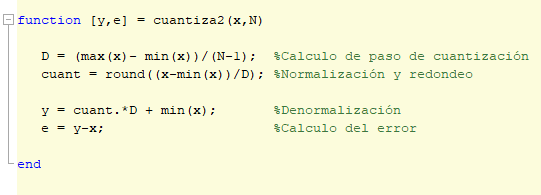
\includegraphics[scale = 0.5]{imagenes2/cuantiza2.png}
        \caption{Implementación de la función \texttt{cuantiza} modificada para entregar señal cuantizada y el error con respecto a la señal original.}
        \label{cuantiza2}
    \end{figure}
    
        
        Al aplicar esta función a los archivos de  audio \texttt{sonidos-de-voz-16-16.wav} y \texttt{musica-16-16.wav} con 4 niveles de cuantización y graficar tanto las señales originales como las cuantizadas  llevadas al mismo rango original se obtienen las gráficas presentes en la figura \ref{original_cuantizada}
        
        \begin{figure}[H]
            \centering
            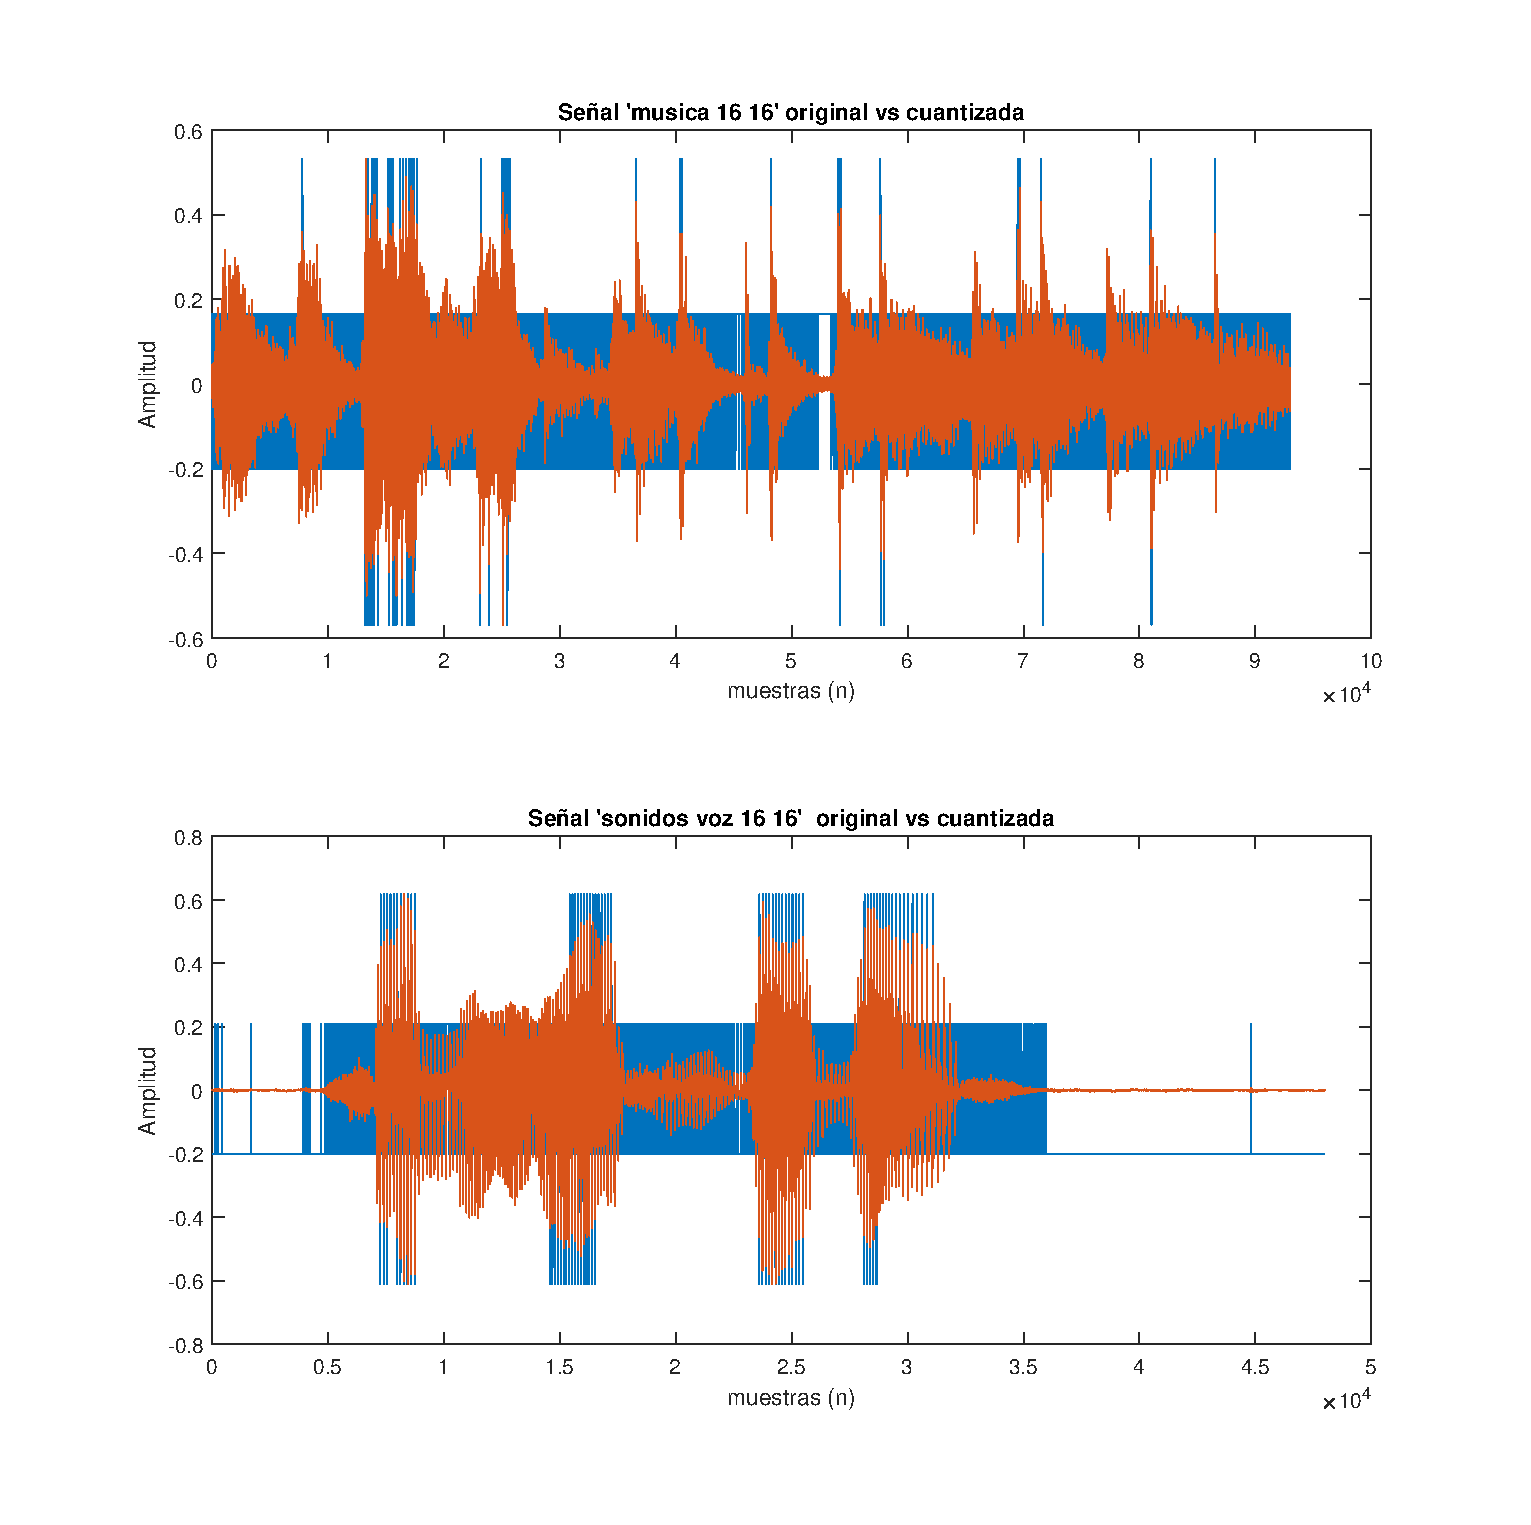
\includegraphics[scale = 0.5]{imagenes2/original_cuantizada.eps}
            \caption{Gráficas comparativas entre los archivos de audio originales y las señales obtenidas de su respectiva cuantización y reescalamiento.}
            \label{original_cuantizada}
        \end{figure}
        
  
        
        %Comentar las graficas
        
    \item Se grafican los histogramas de 20 bins del error para cada señal de audio, \texttt{musica-16-16.wav} y \texttt{sonidos-de-voz-16-16.wav}, para una cantidad de 2 bits, es decir 4 niveles de cuantización. Obteniéndose así las gráficas de la figura \ref{fig:histogramas}
    
    
    \begin{figure}[H]
        \centering
        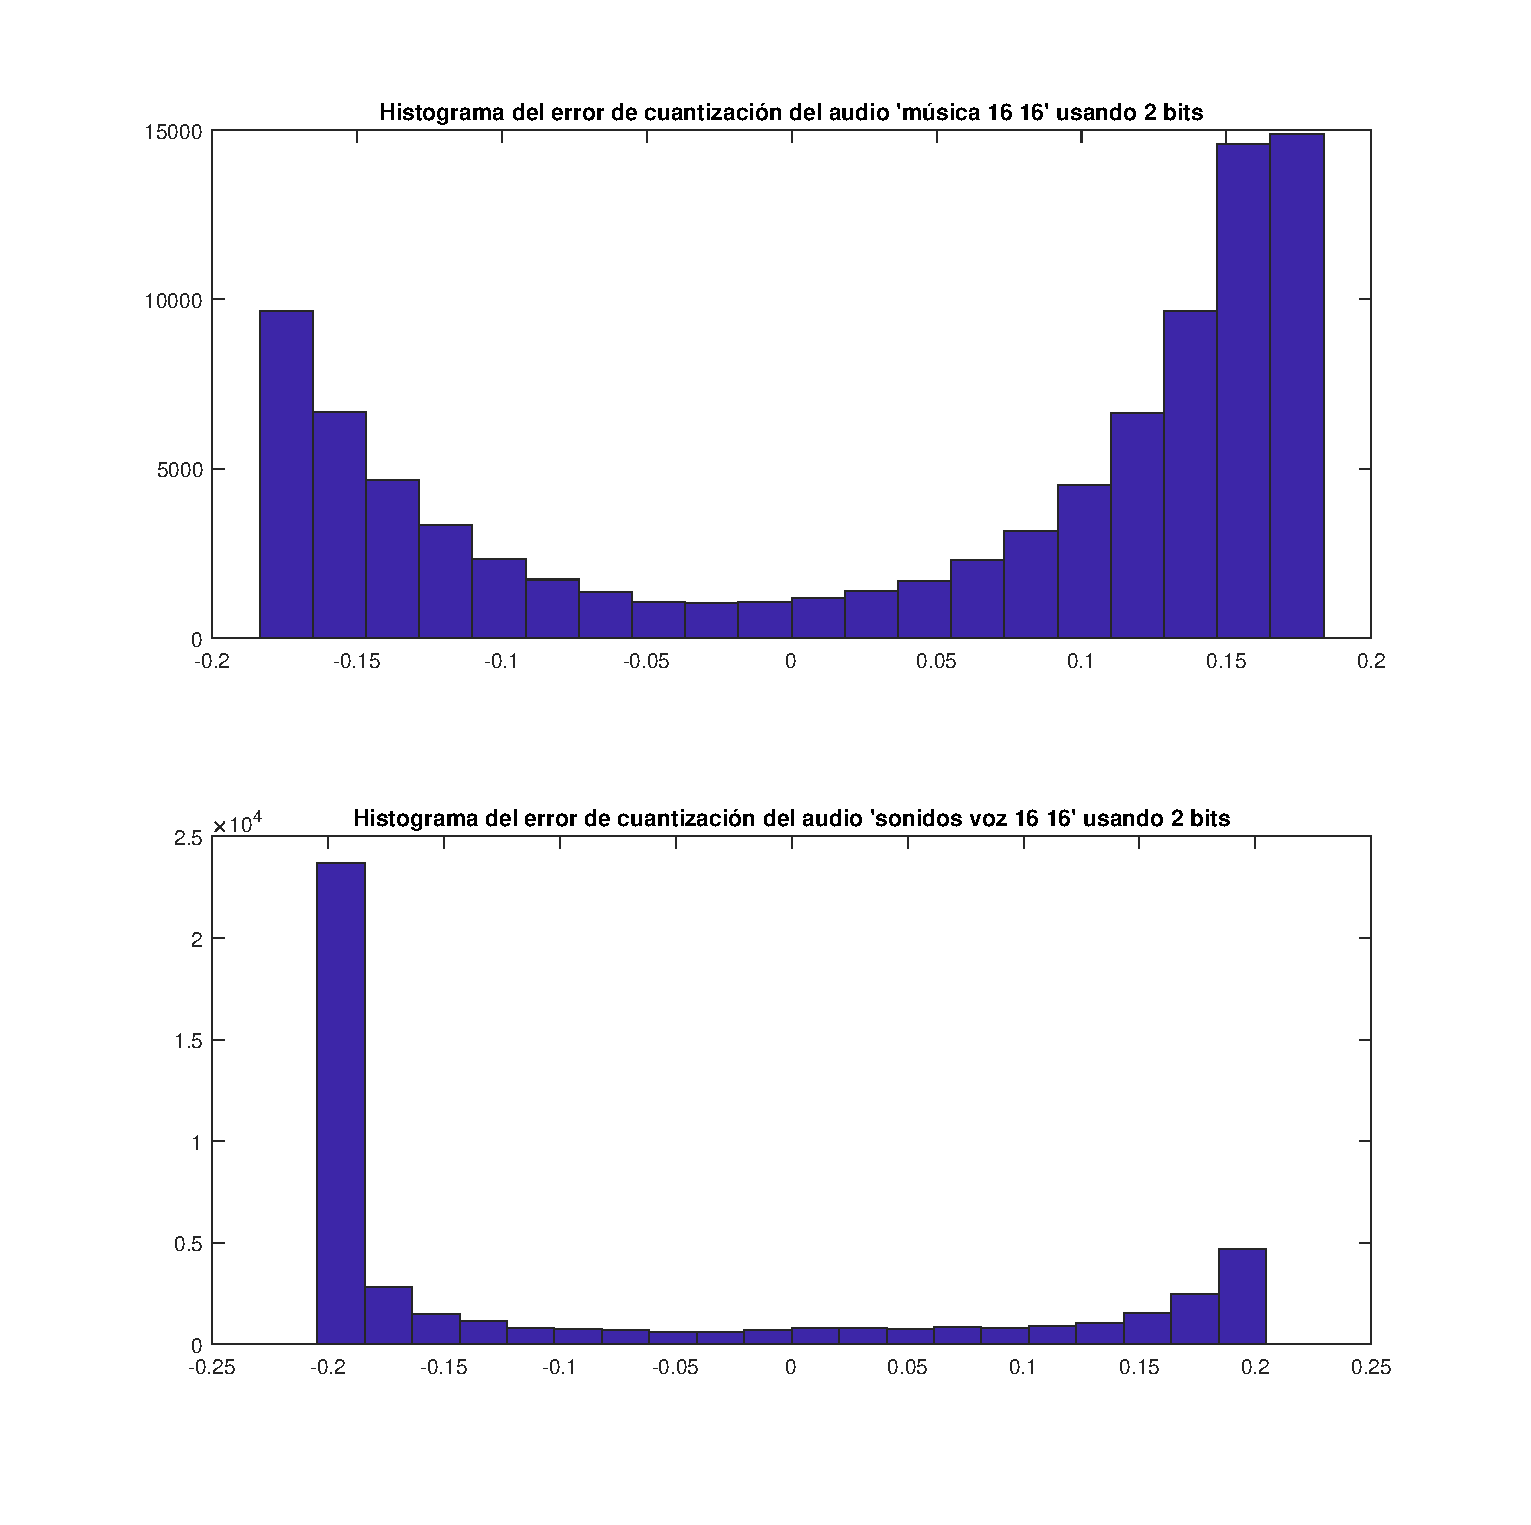
\includegraphics[scale = 0.5]{imagenes2/histogramas.eps}
        \caption{Histogramas del error asociado a la cuantización de las señales de audio  \texttt{musica-16-16.wav} y \texttt{sonidos-de-voz-16-16.wav}.}
        \label{fig:histogramas}
    \end{figure}
    
    Se realizó el proceso de graficar los histogramas del error de cuantización de las señales de audio para 1, 2, 4 , 8 y 12 y 1 bits. Se concluye que si se aumenta la cantidad de bits disponibles en la cuantización, es decir, hay más niveles de cuantización, la gráfica del histograma del error tiene  una distribución cada vez más cercana a la  uniforme,  por lo que el error  (interpretable como ruido en este caso) no está correlacionado con la señal misma. Por otro lado, al reducir la cantidad de bits disponibles, el histograma tiende a concentrarse en los extremos de las gráficas, lejos del cero. Esto es esperable ya que si hay pocos niveles de cuantización es poco probable conseguir errores de magnitud baja debido a que hay pocas opciones de valores para aproximar  el valor de la muestra, pudiendo haber mucha diferencia entre estas dos cantidades.
    
    %%%COrrelación
    \item Se obtiene la autocorrelación del error de cuantización para con diferentes cantidades de bits en el proceso (1, 2, 4, 8 y 12 bits). Además se obtiene la correlación de dicho error con la señal original, en este caso el archivo de audio \texttt{musica-16-16.wav}
    
    Las gráficas comparativas entre la autocorrelación del error de cuantización y la correlación del error con la señal original utilizando 2 y 12 bits se muestran en la figura \ref{fig:xcorr}.
\newpage    
    Con respecto a la autocorrelación del error de cuantización y la correlación con la señal original se puede comentar que:
    \begin{itemize}
        \item A medida que aumenta la cantidad de bits, la autocorrelación del error empieza a parecerse más a un delta de kronecker. Recordando que la DTFT de la autocorrelación corresponde a la Densidad Espectral de Potencia (PSD) y que la DTFT de un delta de kronecker es una constante, se concluye que el error tiene una PSD que tiende a ser plana a medida que aumentan los bits, es decir, empieza a comportarse como ruido blanco.  
        
        \item Se aprecia que al haber pocos bits existe una correlación no despreciable cuando la señal original y la señal de error tienen poco retardo entre ellas. A medida que los bits aumentan la correlación entre la señal original y el error de cuantización tiende a ser cercano a 0 aún cuando hay poco retardo. Lo anterior es un supuesto usual cuando el error corresponde a ruido blanco. 
    \end{itemize}
    
    \begin{figure}[H]
        \centering
        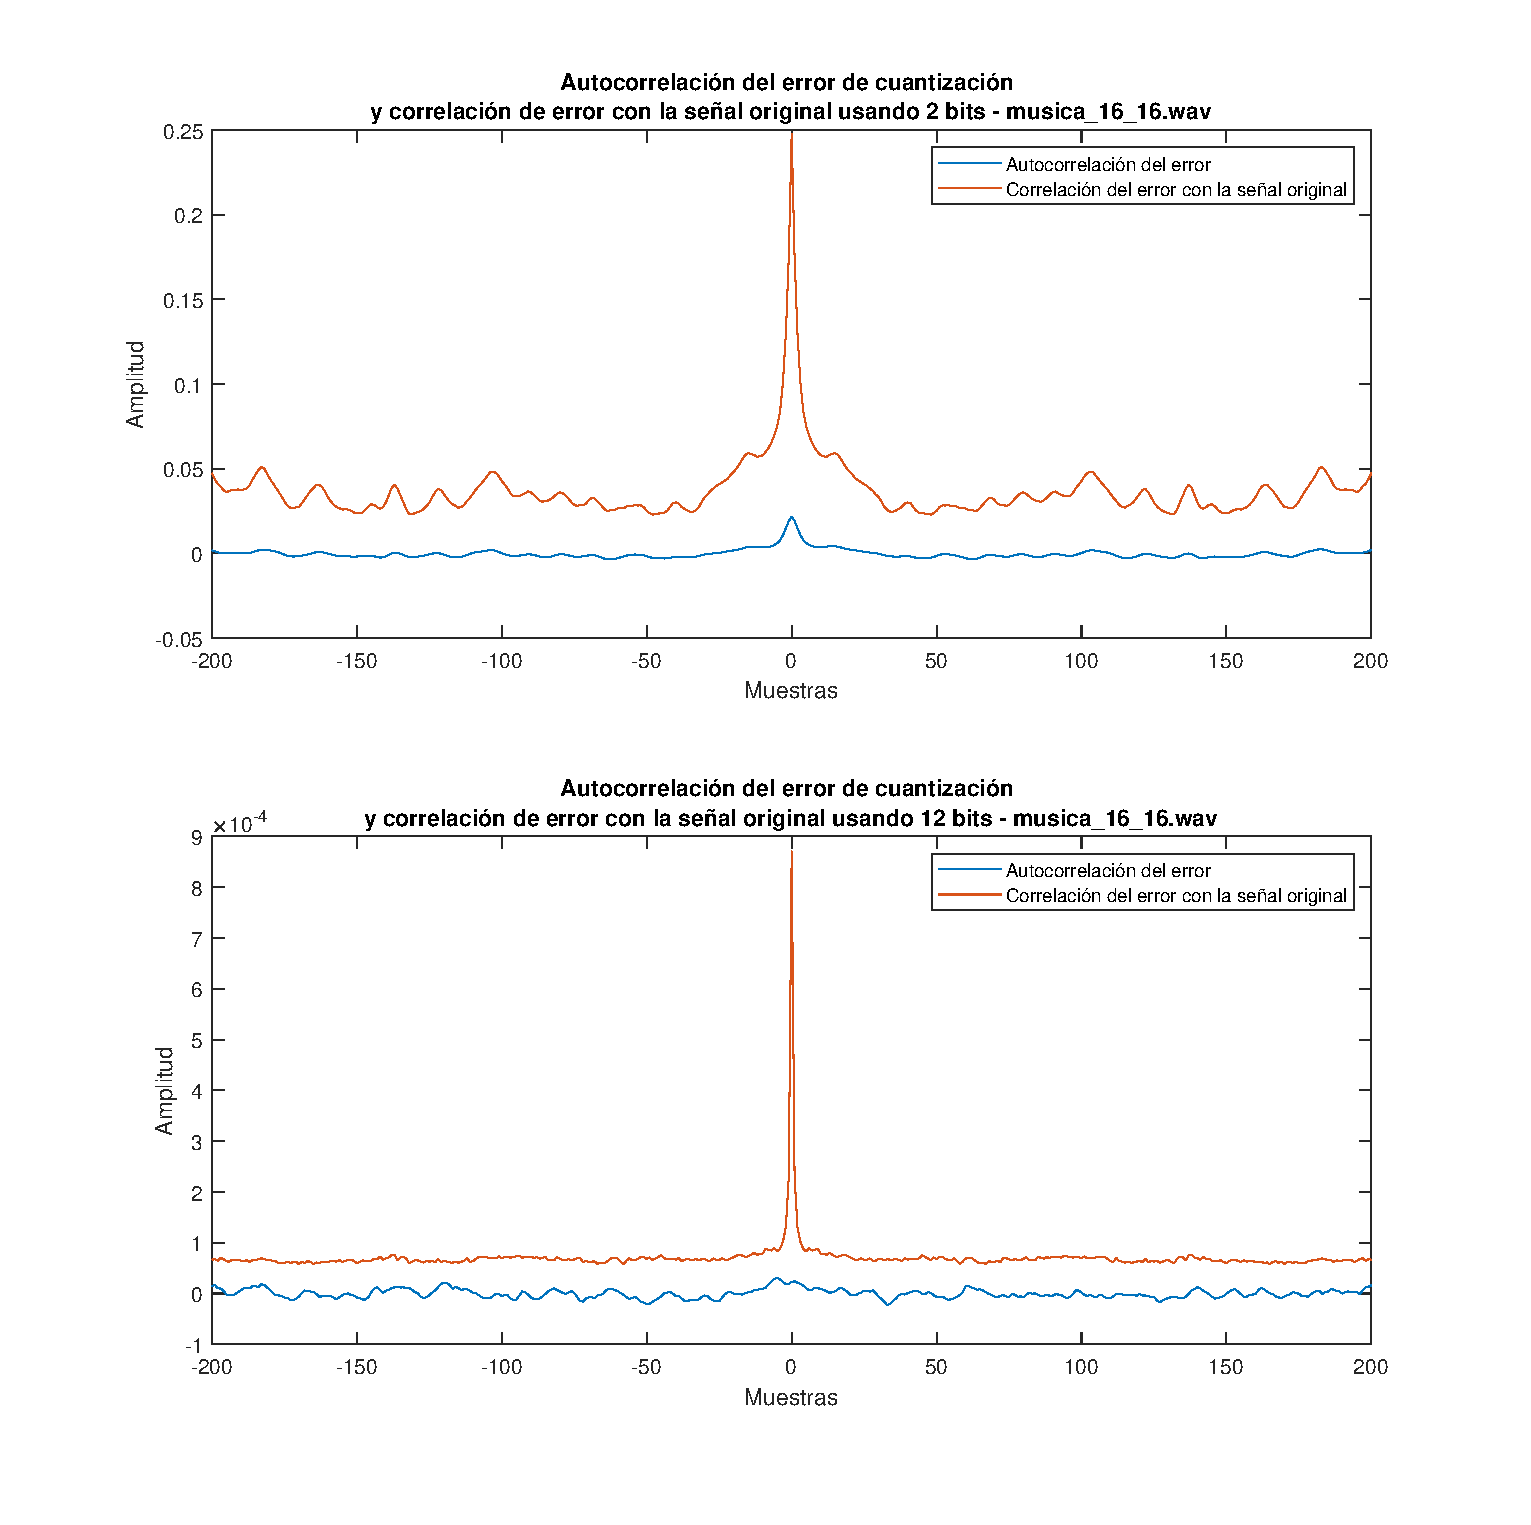
\includegraphics[width = 0.9\linewidth]{imagenes2/xcorr_error.eps}
        \caption{Autocorrelación del error de cuantización y correlación del error con la señal original para 2 y 12 bits}
        \label{fig:xcorr}
    \end{figure}
    
    
    
  \end{enumerate}
  
  
  \item Se modifica nuevamente la función para implementar \texttt{cuantiza-dither(x,N)}, que recibe los mismos parámetros que en los casos anteriores. El propósito de esta función es hacer \textit{Ditherring} a la señal para poder descorreelacionar el ruido de cuantización. Para ello se siguen pasos similares a los realizados en los casos anteriores, pero esta vez a la señal se le agrega ruido blanco o gaussiano con una desviación estándar del $25\%$ del valor de paso de cuantización. El código MATLAB que realiza esta función se encuentra en la figura \ref{dither} 
  
  
  \begin{figure}[H]
      \centering
      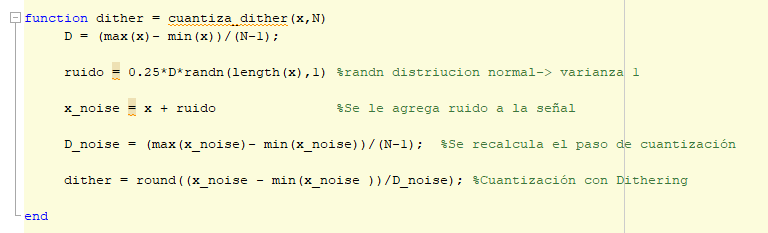
\includegraphics[scale = 0.5]{imagenes2/dither.png}
      \caption{Implementación en MATLAB de la función  \texttt{cuantiza-dither(x,N)}.}
      \label{dither}
  \end{figure}
  
  Al reproducir las señales obtenidas se escucha prácticamente solo ruido, a pesar de el aumento en el número de bits. En el caso de el archivo de música incluso haciendo uso de 12 bits solo se escucha ruido, para el caso del archivo de voz, usando este mismo número de bits se logra apreciar levemente el mensaje de la señal original pero de todas formas opacado casi completamente por el ruido.
  
  Comparando lo escuchado al cuantizar directamente las señales originales y lo que se obtiene al hacer la cuantización cuando se aplica \textit{Dithering}, el sonido es más inteligible al oído en el primer caso, en éste se logra notar claramente la diferencia que se produce en el resultado al modificar la cantidad de bits en la cuantización. Esto no ocurre cuando se aplica \textit{Dithering}.
  
  
    
\end{enumerate}
\subsection{Operación Básica con Punto Fijo}

Para esta sección se considera el caso de aplicar un enventanamiento con una ventana Blackman a un vector de $N=161$ datos de audio. Se supone que se debe operar usando aritmética de punto fijo y que el ADC entrega las muestras cuantizadas como un número entero con signo \texttt{int16}.

\begin{enumerate}[a)]
    \item Se lee el archivo \texttt{aliasing\_test\_16\_16.wav} con su tipo de dato nativo (\texttt{int16}) y se rescatan en la variable $x$ las primeras $N$ muestras.
    
    Notar que al utilizar \texttt{audioread(aliasing\_test\_16\_16.wav)} para leer el archivo de audio se obtiene un vector de datos tipo \texttt{double} de máxima amplitud igual a 1. Comparando con la máxima amplitud de los datos obtenidos al leer el archivo en formato nativo se concluye que el vector de datos corresponde a la representación interna utilizando 16 bits en $Q15$.
    
    \begin{figure}[H]
        \centering
        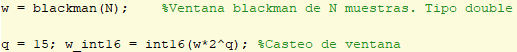
\includegraphics{imagenes2/p6_blackman.png}
        \caption{Código en MATLAB para obtener una ventana Blackman como un vector de datos de 16 bits en $Q15$.}
        \label{fig:p6_blackman}
    \end{figure}
    
    La sección de código para obtener la ventana Blackman como un vector de datos de 16 bits en $Q15$ se muestra en la figura \ref{fig:p6_blackman}. Del código puede comentarse que:
    \begin{itemize}
        \item En la primera línea se obtiene una ventna blackman de $N$ datos, los cuales son de tipo \texttt{double}.
        \item La segunda línea corresponde a la transformación a formato 16 bits $Q15$. Recordar que:
        $$ w = w_{ri}\cdot 2^{-q}$$
        donde $w$ representa la ventana, $w_{ri}$ la ventana en representación interna y $q$ el número de bits que correspoden a decimales.
        
        Como se dispone de la ventana en formato \texttt{double}, se debe despejar $w_{ri}$ para obtener la ventana en 16 bits $Q15$, que es precisamente lo que se hace en la segunda línea. 
    \end{itemize}
    
    Aplicando el comando \texttt{whos} se obtiene que:
    \begin{itemize}
        \item La ventana con datos de tipo \texttt{double} ocupa 1288 bytes.
        \item La ventana con datos de tipo \texttt{int16} ocupa 322 bytes.
    \end{itemize}
    
    Como era de esperarse, se ocupa 4 veces menos memoria, lo cual resulta una mejora considerable asumiendo que se cuenta con hardware para operación en punto fijo.
    
    Posteriormente se aplica el enventanamiento en punto fijo.
    
    \begin{figure}[H]
        \centering
        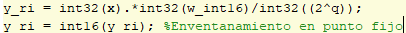
\includegraphics{imagenes2/p6_pond.png}
        \caption{Código en MATLAB para obtener enventanamiento simulando operación en punto fijo.}
        \label{fig:p6_pond}
    \end{figure}
    
    La sección de código para obtener la ventana Blackman como un vector de datos de 16 bits en $Q15$ se muestra en la figura \ref{fig:p6_blackman}. Del código puede comentarse que:
    
    \begin{itemize}
        \item La primera y segunda línea corresponden a la obtención del producto en representación interna. Recordar que
        $$ c = a\cdot b = (a_{ri}\cdot b_{ri}\cdot 2^{-q})\cdot 2^{-q}\Rightarrow c_{ri} = a_{ri}\cdot b_{ri}\cdot 2^{-q}$$
        donde el $ri$ hace referencia a la representación interna en $Qq$, siendo $q$ el número de bits correspondientes a decimales.
        
        Con lo anterior resulta claro que la primera línea corresponde a la obtención en representación interna de $y$, donde se trabaja con datos \texttt{int32} por el overflow de la multiplicación. En la segunda se vuelve al tipo de dato \texttt{int16}. 
    \end{itemize}
    
    Aplicando el comando \texttt{whos} se obtiene que:
    \begin{itemize}
        \item El enventanamiento (ponderación) con datos de tipo \texttt{double} ocupa 1288 bytes.
        \item El enventanamiento (ponderación) con datos de tipo \texttt{int16} ocupa 322 bytes.
    \end{itemize}
    
    obteniendo nuevamente un factor de 4 veces menos memoria al operar con datos \texttt{int16}. 
    
    Finalmente se obtiene una representación gráfica de la señal $x$, $w$ e $y$ en representación interna, la cual aparece en la figura \ref{fig:p6_graf}. Visualmente se aprecia la ponderación es correcta.
    
    \begin{figure}[H]
        \centering
        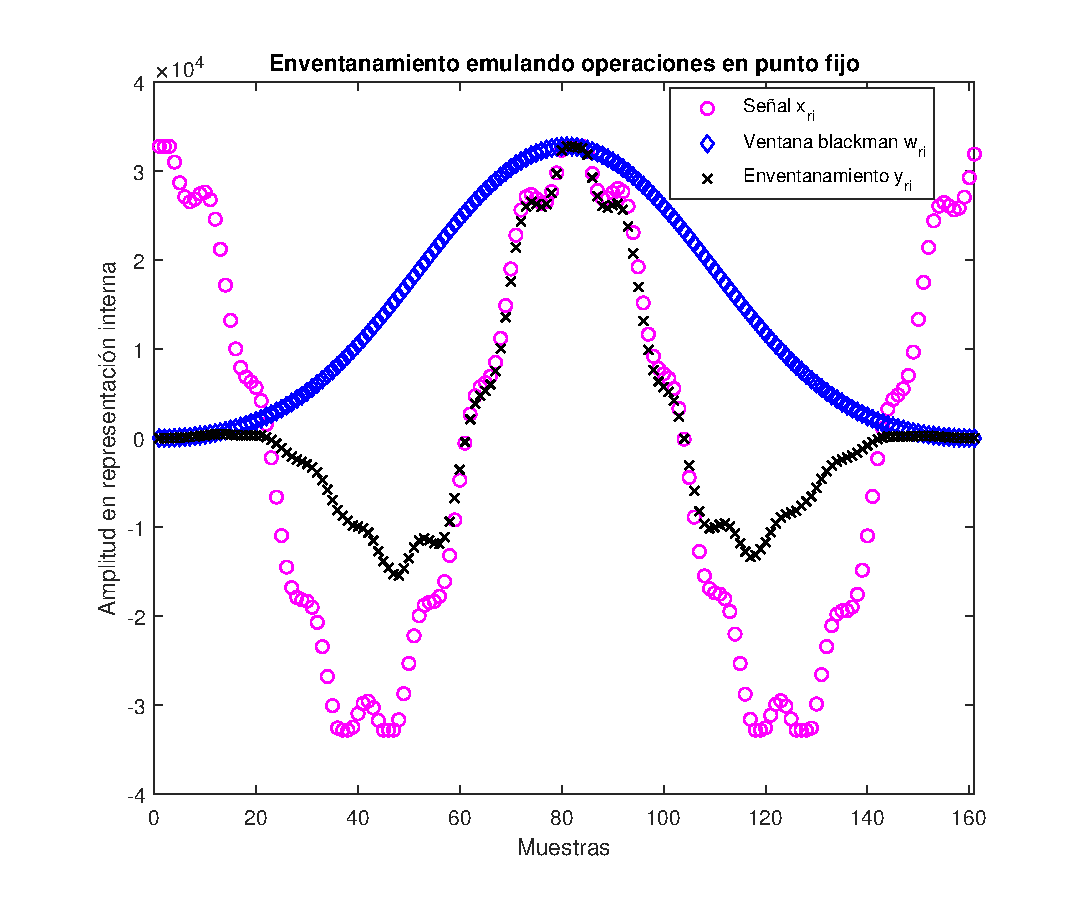
\includegraphics[width = .9\linewidth]{imagenes2/p6_graf.eps}
        \caption{Señales $x$, $w$ e $y$ en representación interna vs muestras.}
        \label{fig:p6_graf}
    \end{figure}
    
\end{enumerate}


















\end{document}

